\documentclass{umthesis}          % for Ph.D. dissertation or proposal

% CLRSCode is for pseudocode
% See http://www.cs.dartmouth.edu/~thc/clrscode/
\usepackage{clrscode3e}
\usepackage{graphicx}
\usepackage{amssymb}
\usepackage{url}
\usepackage{lscape}

% This width is used for many figures  -- Curran August 2014
\newcommand{\figureWidth}{6in}

\begin{document}
\title{Visualizing the\\Universal Data Cube}
\author{Curran Kelleher}
\date{September 2014}
\copyrightyear{2014}
\bachelors{B.Sc.}{University of Massachusetts Lowell}
\masters{M.Sc.}{University of Massachusetts Lowell}

\committeechair{Dr. Haim Levkowitz}
\firstreader{Dr. Jesse Heines}
\secondreader{Dr. Rosane Minghim}
\departmentchair{Dr. Jie Wang}
\departmentname{Computer Science}

\degree{Doctor of Philosophy}{Ph.D.}
%% These lines produce the title, copyright, and signature pages.
%% They are Mandatory; except that you could leave out the copyright page
%% if you were preparing an M.S. thesis instead of a PhD dissertation.
\frontmatter
\maketitle
\copyrightpage     %% not required for an M.S. thesis
\signaturepage

%%
%% Dedication is optional -- but this is how you create it
%% \begin{dedication}              % Dedication page
%%   \begin{center}
%%     \emph{To Nita.}
%%   \end{center}
%% \end{dedication}

%%
%% Epigraph goes here...(aka frontispiece)
%% \chapter{Epigraph}?????

%%
%% Acknowledgements are optional...yeah, right.
\chapter{Acknowledgments}             % Acknowledgements page
I would like to thank my parents Daniel and Marcella Kelleher and my brother Sean for supporting me throughout my education. I am grateful to my committee members Dr. Haim Levkowitz, Dr. Rosane Minghim, and Dr. Jesse Heines for their support and feedback throughout the dissertation process. I would also like to acknowledge Dr. Georges Grinstein and Dr. Daniel Keim for their mentorship and support of my work in its early stages.

\begin{abstract}
The field of data visualization is lacking open tools that support easily developing and using production quality interactive visualizations. Particularly, there is a need for reusable solutions for (1) well known visualization and interaction techniques (2) authoring and sharing visualizations with multiple linked views, and (3) describing existing data such that many data sets can be easily integrated and visualized. This dissertation introduces novel data structures and algorithms for interactive visualizations of data from many sources, addressing these three issues.
\end{abstract}

%%
%% Preface goes here...would be just like Acknowledgements -- optional
%% \chapter{Preface} 
%% ...


%%
%% Table of contents is mandatory, lists of tables and figures are 
%% mandatory if you have any tables or figures; must be in this order.
\tableofcontents                % Table of contents
\listoftables                   % List of Tables
\listoffigures                  % List of Figures

%%
%% We don't handle List of Abbreviations
%% We don't handle Glossary

%%%%%%%%%%%%%%%%%%%%%%%%%%%%%%%%%%%%%%%%%%%%%%%%%%%%%%%%%%%%%%%%%%%%%%%%%
%% Time for the body of the dissertation
\mainmatter   %% <-- This line is mandatory

%\unnumberedchapter{Introduction}
\chapter{Introduction}
The contributions of this dissertation are novel data structures and algorithms for integration and interactive visualization of many data sets from multiple sources, based on the data cube concept. The proposed data representation framework will allow data sets to be combined together and visualized using interactive visualization dashboards like the one described above, giving users the sense that the data exists within a single unified structure. The framework is designed to be able to represent and integrate an arbitrary number of data sets created independently of one another, and expose the integrated structure to reusable visualization tools that can be combined together in dashboard layouts with multiple linked views using existing interaction techniques such as brushing and linking. The proposed data representation and visualization framework is fundamentally new, and will allow heterogeneous data sets to be explored in a unified way that was never before possible. 

The overall goal of this work is to build digital telescope into the universe of phenomena on Earth via publicly available data. For example, consider public data sources such as the United Nations, the US Census, the US Bureau of Labor Statistics, or the US Centers for Disease Control. These organizations and hundreds of others around the world provide publicly available data about various topics including population statistics, public health, distribution of wealth, quality of life, economics, the environment, and many others. By unifying these data sources and providing users with tools to explore and present the data visually, a deeper understanding of the world can be gleaned through the lens of public data. The focus of this dissertation is on applications involving public data, however the techniques introduced can be applied to any data sets that can be conceptually modeled as data cubes, regardless of whether they are public or private. 

Consider the data from the US Census that covers population statistics for US States from 1950 to 2010. Consider also population statistics from the United Nations covering World Countries from 1970 to 2012. These two data sets may use different identifiers for years and geographic regions, but they cover an overlapping conceptual data space of time, geography and population. From these two data sets it is possible to create a visualization dashboard with a map of the world showing population as color and a corresponding line graph showing population for each region as lines. If the user views the whole world, the UN population data is shown for each country. If the user zooms into the US, US Census data is shown for each state. If the user selects a point of time in the line graph, the data shown on the map is from that point in time. If the user pans and zooms on the map, the lines in the line graph update to only show the regions visible on the map. This is one example of an interactive visualization dashboard with multiple linked views (the timeline and map views) operating over multiple data sets integrated from different sources (the United Nations population data and the US Census population data).

\TODO{implement this and put screenshot image here}

Data cubes, also known as OLAP (OnLine Analytical Processing) cubes, can represent data that contains measures aggregated (typically using sum or average) along categorical hierarchies. The data cube concept emerged from the field of data warehousing as a way to summarize transactional data, allowing analysts to get a bird's eye view of company activities. The term OLAP stands in contrast to the term OLTP (OnLine Transaction Processing), which is the part of the data warehouse system that ingests and stores data at the level of individual transactions or events. After the ETL (Extract, Transform and Load) phase of the data warehouse flow, the data is analyzed by computing a data cube from the transactional data.

The data cube concept and structure can be used to model existing data sets as well. Publicly available data sets (often termed ``statistical data'') may be considered as pre-computed data cubes if they contain aggregated measures (also called ``indicators'', ``metrics'' or ``statistics'') across time, geographic space or other dimensions such as gender, age range, ethnicity or industry sector. Any categorization scheme containing distinct entities, organized as an unorered collection, an ordered collection, or a hierarchy can be modeled as a dimension. Any numeric value that represents an aggregated statistical summary using sum, average, or other aggregation operator can be modeled as a measure.

With this approach, it is possible to model many data sets together using shared dimensions and measures. This will allow integration of many data sets together in a single unified structure. Existing data cube technologies assume that data cubes will be computed from a relational source, and are not designed to handle integration of pre-computed data cubes that may use inconsistent identifiers for common dimensions and inconsistent scaling factors for common measures. Therefore the application of the data cube concept to integration and visualization of many pre-computed data cubes, while theoretically plausible, requires the development of novel data structures and algorithms that extend the data cube model to handle integration of pre-computed data cubes that may use inconsistent identifiers for common dimensions and inconsistent scaling factors for common measures.

The data cube structure lends itself particularly well to visualization. Long standing perception-based data visualization theory presented by Bertin \cite{bertin1983semiology} and Mackinlay \cite{mackinlay1986automating} identify effective ways to visually encode data based on data fields that are nominal, ordinal or quantitative. Visualization techniques have been explored for hierarchical (tree-based) data as well \cite{graham2010survey}. Data cubes can contain data of these types. Therefore existing visualization theory can be applied to the data cube model to determine which visualizations are appropriate for representing which data, depending on its data cube structure. This topic is discussed in section \ref{dataCubeVisualization}.

\pagebreak
\section{Related Work}
Previous work relating to this dissertation falls into four major categories:
\begin{itemize}
\item data representation - structures, models and formats for data
\item data integration - merging data from many sources
\item data visualization - transforming data into interactive graphics
\item Web graphics technology - HTML5 graphics APIs and libraries
\end{itemize}
\subsection{Data Representation}
%In today's world of ``information overload'', data takes many forms. Perhaps the most familiar data representation system today is Microsoft Excel, which is capable of representing data tables as well as complex operations across the data values \cite{eick2000visualizing}. Many organizations use Excel to manage data or make data available as Excel spreadsheets. For example, the United Nations Department of Economic and Social Affairs makes their population statistics available in Excel format (see figure \ref{fig:unPopExcel}).
%
%\begin{figure}[h!]
%  \centering
%  \includegraphics[width=\textwidth]{figures/UN_World_Population_Spreadsheet.png}
%  \caption[United Nations population estimates spreadsheet.]
%   {The United Nations Population Prospects data set \cite{unPopData}, made available in Excel format. This is another example of a public data set that could be imported into our data representation framework.}
%  \label{fig:unPopExcel}
%\end{figure}
%
Relational database systems provide a mature data management solution and are widely adopted \cite{ramakrishnan2000database}. The relational model has well understood theoretical underpinnings such as relational algebra \cite{clifford1985algebra}. Data warehouse systems are typically built on the relational model and are augmented by multi-scale aggregated data structures called data cubes, also known as OLAP (OnLine Analytical Processing) cubes \cite{gray1997data, codd1993providing}. Data cubes contain summaries of the collection of facts stored in a relational database \cite{chaudhuri1997overview}. For example, a data cube may contain how much profit was made from month to month subdivided by product category, while the relational database may contain the information associated with each individual transaction.

Because data cubes provide an abstraction that handles aggregation, they are a widely used method of data abstraction for supporting visualization and analysis tasks \cite{stolte2003multiscale}. Kimball pioneered the area of ``Dimensional Modeling'', which concerns constructing data warehouse schemas amenable to data cube construction and analysis \cite{kimball1998data}. Data cubes have been implemented in a variety of different systems, so effort has been made to discover unified conceptual or mathematical models that can characterize many implementations \cite{datta1999cube, vassiliadis1999survey, vassiliadis1998modeling, li1996data, agrawal1997modeling, gyssens1997foundation, blaschka1998finding}. The data cube structure has also been used to model user Web browsing sessions to support data mining algorithms for Web prefetching \cite{yang2003data}.
%
%NoSQL systems are modern databases that are designed to go beyond the scalability limitations of relational systems \cite{cattell2011scalable}. While NoSQL systems sacrifice some of the integrity constraints upheld by relational database systems \cite{stonebraker2010sql}, they are gaining traction in industry because they can handle the scale of data demanded by applications of the ``Big Data'' era \cite{leavitt2010will}. NoSQL systems provide flexible storage systems that do not necessarily require the definition of a schema. This makes it arguably easier to modify and update the type of content stored over time as compared to relational systems.
%
%The Semantic Web is a vision of a ``Web of Data'' coexisting with the World Wide Web \cite{berners2001semantic}. The basis of the Semantic Web is the RDF (Resource Description Framework) data model, which represents a graph of data in the form of (subject, predicate, object) triples. The Semantic Web vision has evolved into the concept of Linked Data, which refers to data that is available as RDF and made available according to common conventions \cite{bizer2009linked} \cite{bizer2007publish}. Any data that can be represented using a relational database can also be represented using RDF \cite{bizer2006d2r}. The SPARQL query language for RDF can be used to query and integrate data from multiple sources \cite{quilitz2008querying}. Lopez et al. developed an information management system for integrating and analyzing heterogeneous information sources characterizing urban areas \cite{lopez2012queriocity}. The Semantic Web technology stack contains a method for declaring when different identifiers refer to the same entity and processing queries appropriately to integrate data \cite{halpin2010owl} \cite{ding2010sameas}. While the Semantic Web provides a compelling vision, its adoption is not as widespread as one might expect \cite{lytras2008semantic}.
%
%The RDF Data Cube Vocabulary is capable of representing data cubes using Semantic Web technologies \cite{rdfdatacube}. The intention of the RDF Data Cube Vocabulary is to provide a common representation and interchange format for statistical data. The RDF Data Cube Vocabulary draws from a previous effort called the Statistical Data and Metadata eXchange (SDMX) initiative that was launched in 2001 by seven organizations working on statistics at the international level \cite{cyganiak2010semantic}. The primary challenges faced when using the RDF Data Cube Vocabulary include transforming to and from well known formats and data models. Salas et al. discussed how data can be transformed from existing OLAP systems or flat files into RDF using the Data Cube Vocabulary, and also introduced a faceted visualization tool for RDF data cubes \cite{salas-icsc-2012}. K{\"a}mpgen et al. investigated how data represented using the RDF Data Cube Vocabulary can be transformed for analysis using traditional OLAP systems \cite{kampgen2011transforming}. Maali et al. proposed a pipeline for converting government data into high quality Linked Data utilizing the Data Cube Vocabulary \cite{maali2012publishing}.
%
%Datta et al. introduce a conceptual model for data cubes \cite{datta1999cube}. In this formalization, a data cube (or, in the terms of the authors, a data cube instance) is defined as a 6-tuple $(D, M, A, f, V, g)$ where $D$ is a set of dimensions, $M$ is a set of measures, $A$ is a set of attributes, $f$ is a function that maps dimensions to sets of attributes (the levels of the dimension), $V$ is a set of tuples that assign concrete numeric values for each measure, and $g$ is a function that maps data cube cells to tuples in $V$. The authors formalize common OLAP operators including slice, drill-down, roll-up, and pivot, as well as operators over multiple cubes including join, union, intersection and difference. This formalism captures the essence of data cubes, but is limited in that it does not deal with integrating data cubes from multiple sources where names used for dimensions, attributes and measures may not match.
%
%Kuznetsov et al. introduce a mathematical formalism of data cubes based on lattice theory \cite{kuznetsov2009mathematical}. This work focuses primarily on characterizing the lattice structure of hierarchical data cubes and relating the structure to established mathematics in lattice theory. The contribution of this work is primarily mathematical, and the structures introduced do not cover the entire problem area of representing, structuring and querying complete data cubes. This characterization is similar to the zoom graph concept introduced by stolte et al. \cite{stolte2003multiscale}. Usman et al. introduced a conceptual model for OLAP enhanced for coupling with data mining and visualization techniques \cite{usman2009conceptual}.
%
\subsection{Data Integration}
%The field of data integration offers many techniques for combining data from multiple sources based on the relational model \cite{doan2012principles} as well as from a theoretical perspective \cite{lenzerini2002data} \cite{halevy2006data} \cite{ziegler2004three}. Schema matching is the area of data integration that concerns semantic matching between the attributes of data tables from different sources \cite{rahm2001survey} \cite{fagin2003data}. Schema matching may be performed manually, however it must be automated in order to scale to hundreds or thousands of different sources. Numerous approaches for automated schema matching have been proposed \cite{shvaiko2005survey} \cite{doan2001reconciling} \cite{kang2003schema} \cite{milo1998using} \cite{madhavan2001generic} \cite{doan2000learning}. Schema matching approaches aimed specifically at Web and Ontology based data integration have also been proposed \cite{he2003statistical} \cite{noy2004semantic} \cite{doan2005semantic} \cite{madhavan2007web} \cite{kalfoglou2003ontology} \cite{noy2009ontology} \cite{uschold2004ontologies} \cite{wache2001ontology} \cite{noy2003prompt} \cite{euzenat2007ontology}. Data matching (also known as record linkage) is the area of data integration focusing on resolving different identifiers to the same real-world entity \cite{winkler1999state} \cite{winkler2006overview} \cite{koudas2006record} \cite{aizawa2005fast} \cite{gu2003record}. Record linkage has been applied extensively to public data \cite{jaro1995probabilistic} \cite{jaro1989advances} \cite{holman1999population}. Several tools have been introduced that aid users in data integration tasks via a graphical user interface \cite{christen2008febrl} \cite{kandel2011wrangler} \cite{elfeky2002tailor}. Techniques from both of these areas must be applied in order to integrate data sets from multiple sources and utilize our proposed unified data model.
%
\subsection{Data Visualization}
%The field of information visualization offers several compelling theoretical approaches for visualizing data. Arguably the first significant work concerning data visualization was William Playfair's ``Commercial and Political Atlas'', published in 1786 \cite{playfair1786commercial}. In this work, Playfair introduced the Bar Chart, Pie Chart, and Line Graph. The first attempt at a systematic formalization of data visualization was Jacques Bertin's ``Semiology of Graphics'' \cite{bertin1983semiology}. In this work, Bertin relates data types to visual marks and channels in a coherent system that takes visual perception into account. Bertin's work has influenced many future theoretical underpinnings of visualization, including Leland Wilkinson's ``Grammar of Graphics'' \cite{wilkinson2005grammar} and Jock Mackinlay's APT (A Presentation Tool) system \cite{mackinlay1986automating}, which led to the development of the commercial visualization package Tableau \cite{hanrahan2007visual}.
%
%As a more concrete manifestation of visualization theory, much effort has been placed on generating taxonomies of visualization techniques. Chi et al. introduced a concrete taxonomy of visualizations \cite{chi2000taxonomy} based on the Data State Reference Model \cite{chi1998operator}. Shneiderman introduced a more general taxonomy based on tasks and data types \cite{shneiderman1996eyes}. Card et al. made steps toward characterizing the entire design space of data visualizations based on Bertin's theory \cite{card1997structure}. Tufte explored numerous visualization techniques for quantitative information in general, many of which can be applied to visualization of data cubes \cite{tufte1983visual}.
%
%Much work has been done regarding visualization of data cubes. Stolte et al. introduced a formalism for defining multi-scale visualizations of data cubes throughout their work on the Polaris system \cite{stolte2003multiscale} \cite{stolte2002query} \cite{stolte2002polaris}. In this work the authors introduce theoretical underpinnings of a visualization system capable of navigating hierarchical data cubes with a combination of data abstraction and visual abstraction. One fundamental concept in this system is the ``zoom graph'', a lattice of data cubes that supports arbitrary interactive zoom paths through the multidimensional data cube hierarchies. Cuzzocrea et al. surveyed the area of data cube visualization in depth \cite{cuzzocrea2009olap} and have made several contributions regarding semantics-aware OLAP visualization \cite{cuzzocrea2007semantics} and a hierarchy driven compression technique for OLAP visualization \cite{cuzzocrea2006hierarchy}. Mansmann coined the term ``Visual OLAP'', framed it as a fundamentally new paradigm for exploring multidimensional aggregates \cite{mansmann2008visual}, explored applications of hierarchical visualization techniques to OLAP cubes \cite{mansmann2007exploring} and extended Visual OLAP to support irregular hierarchies \cite{mansmann2006extending}. Scotch et al. developed and evaluated SOVAT, a Spatial OLAP visualization and analysis tool applied to community health assessments \cite{scotch2005sovat} \cite{scotch2007usability}. Lee and Ong introduced a visualisation technique for knowledge discovery in OLAP combining elements of bar charts and parallel coordinates \cite{lee1995new}. Maniatis et al. explored how OLAP cubes can be visualized using TableLens and other techniques \cite{maniatis2003advanced}. Data cubes have also been utilized as the foundational data structure for several ``Big Data'' visualization systems \cite{lins2013nanocubes} \cite{liu2013immens}.
%
%Interactions within data visualization environments have been well studied. Becker et al. investigated brushing in scatter plots \cite{becker1987brushing}. Shneiderman et al. explored dynamic queries in general and how these operations fit into a larger context of visual information seeking \cite{shneiderman1994dynamic}. Ward introduced a visualization system based on multiple linked views with direct manipulation techniques including brushing and linking \cite{ward1994xmdvtool}. Anselin discussed how interactive visualization systems with linked views can be applied to Geographic Information Systems \cite{anselin1999interactive}. Yi et al. conducted a thorough survey of existing taxonomies for visualization and interactions and developed a set of generalized classes of interactions for visualization \cite{yi2007toward}. Techapichetvanich et al. explored how visualization interactions pertain to OLAP cubes in particular \cite{techapichetvanich2005interactive}. Sifer et al. introduced a visual interface utilizing coordinated dimension hierarchies for OLAP cubes \cite{sifer2003visual}. Tegarden formulates some requirements for information visualization relevant for business applications, and highlights some unconventional interactive visualizations with potential application to data cube visualization \cite{tegarden1999business}.
%
\subsection{Web Graphics Technology}
%
%The World Wide Web has evolved to become a full fledged application development platform. HTML5 is the latest set of standards and APIs (Application Programming Interfaces) from the World Wide Web Consortium that define the capabilities of modern Web browsers \cite{html5}. HTML5 applications are able to run across multiple platforms (albeit requiring some effort from developers). HTML5 has eclipsed Java Applets and Flash in fulfilling the dream of ``write once, run anywhere''. HTML5 contains three graphics technologies that can support interactive Web-based visualizations: Canvas, SVG (Scalable Vector Graphics), and WebGL.
%
%HTML5 Canvas provides a 2D immediate mode graphics API \cite{fulton2013html5}. When using the Canvas API, developers must work with a stateful graphics context by issuing commands to manipulate the raster image of a Canvas element within the HTML page. This approach requires developers to manage rendering logic at a low level and manage data structures that correspond to graphical representations. The Canvas API has seen wide adoption for HTML5-based games, however for visualization applications the higher level SVG API has seen wider adoption.
%
%SVG (Scalable Vector Graphics) provides a 2D retained mode Graphics API \cite{svg}. SVG uses the HTML DOM (Document Object Model) to represent the definition of persistent graphical elements. When using SVG, developers need only be concerned with updating the DOM. The SVG engine within the browser is responsible for updating the display to correspond with the SVG DOM. In this way, SVG is a higher level API than Canvas. This makes SVG a preferred platform for developing visualizations. However, SVG is less optimizable than Canvas, because developers do not have access to the rendering logic at all. SVG has performance limitations relating to performance limitations and DOM manipulation overhead.
%
%WebGL provides a 3D graphics API that is essentially an interface to OpenGL ES \cite{matsuda2013webgl}. OpenGL ES is a subset of OpenGL designed for use in embedded systems and mobile devices. Developers using WebGL must use programming techniques inherited from OpenGL such as buffer management, vertex management, shader definition, 3D projection, and lighting techniques. WebGL enables developers to take advantage of the GPU (Graphics Processing Unit) for massively parallel computation using shaders. WebGL supports high performance 2D and 3D graphics, but is much more complicated to use than Canvas or SVG.
%
%Many high level libraries have been built for supporting use of Canvas, SVG, and WebGL. Three.js is a 3D scene graph library that includes rendering engines for all three graphics technologies \cite{cabello2010three}. Highcharts is a high level visualization library that provides pre-packaged chart types that can be customized to a limited extent. Leaflet is a library for creating tile-based geographic maps with zooming and panning. hBrowse is a generic framework introduced for Web-based hierarchy visualization \cite{kokoszkiewicz2012hbrowse}. Processing.js is a JavaScript port of the graphics language Processing using HTML5 Canvas. Many more libraries for Web-based graphics and visualization exist, but none have come close to the widespread adoption of D3.js.
%
%D3.js is a flexible and powerful visualization library that uses SVG and has a strong community of users \cite{d3}. D3 at its core is a DOM manipulation library with heavy use of functional programming. D3 allows concise declarative statements to define the core logic of visualizations. D3 provides additional APIs for performing common visualization tasks such as defining and using scales, generating labeled axes, and computing layouts from graphs and trees. D3 is at the center of a vibrant developer ecosystem and has seen wide adoption in industry. There are plentiful examples of D3.js usage for creating visualizations, some of which are shown in figure \ref{fig:d3basic}. Many supporting libraries have been created including NVD3 reusable charts, Chart.js for composing visualization elements, Crossfilter.js for interactive multidimensional filtering, and DC.js for multiple linked views.
%
%\begin{figure}[h!]
%  \centering
%  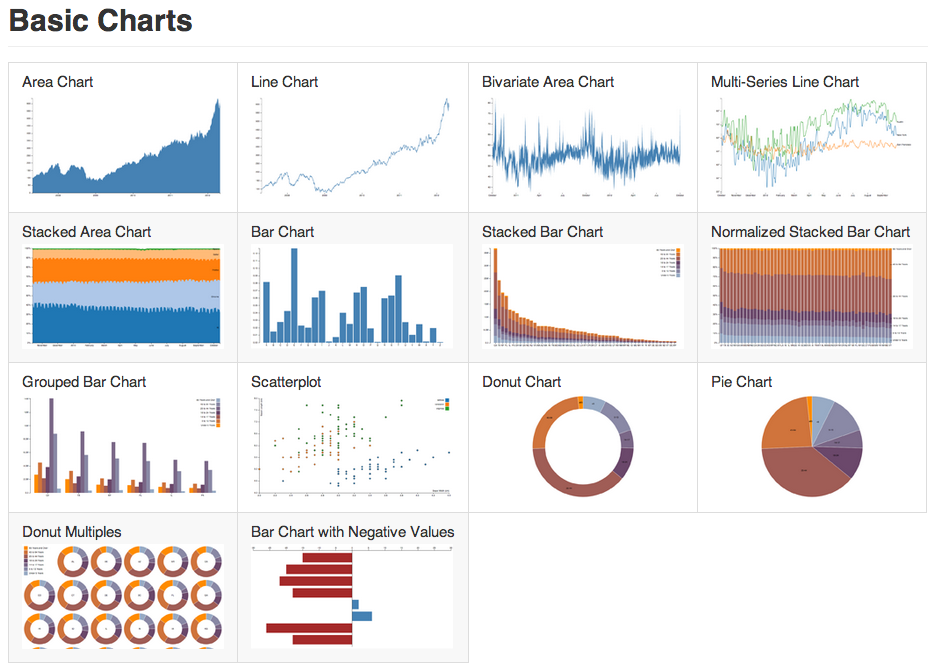
\includegraphics[width=\textwidth]{figures/d3BasicCharts.png}
%  \caption[D3.js basic charts.]
%    {Basic chart examples using D3.js. These are some examples of visualizations that can be tailored to visualize and interact with data cube projections in a generalized manner, building on our proposed framework.}
%  \label{fig:d3basic}
%\end{figure}
%
%Several projects have focused explicitly on visualization of public data on the Web. ManyEyes was an experiment in scaling the audience for visualizations by empowering users to create visualizations of their own data \cite{viegas2007manyeyes}. ManyEyes provided a fixed set of pre-packaged visualization tools and allowed users to visualize their own data tables using the provided visualizations. GapMinder is a project aimed at exposing public data (primarily the United Nations Millenium Development Goals Indicators) using visualization \cite{rosling2005new}. GapMinder includes an animated scatter plot with an interactive time slider, a line chart showing statistics over time, and a world map (see figure \ref{fig:gapminder}). The Google Public Data Explorer provides a visual interface to selected public data sets similar to GapMinder, however it does not make the data available to users in a machine-readable format.
%
%\begin{figure}[h!]
%  \centering
%  \includegraphics[width=\textwidth]{figures/gapminder.jpg}
%  \caption[GapMinder and Hans Rosling.]
%   {Gapminder, a public data visualization tool based on an animated scatter plot, timeline, and map. Here, Professor Hans Rosling, the creator of GapMinder, is shown gesturing the motion of the plot while presenting the visualization.}
%  \label{fig:gapminder}
%\end{figure}
\TODO{pull all related work from proposal}


\chapter{Reactive Visualizations}
Managing complex data flows and update patterns is one of the most difficult challenges in interactive data visualization. Constructing interactive visualizations with multiple linked views can be a daunting task. Functional reactive programming provides approaches for specifying data dependency graphs declaratively and maintaining them automatically. Functional reactive programming can be combined with the Model View Controller (MVC) paradigm to provide reactive models, an effective abstraction that supports construction of complex interactive data visualization systems.

Even with the wealth of visualization toolkits and libraries that exist today, there is a need for an abstraction that addresses the core issue of managing complex data flows and update propagation patterns. In this chapter, a novel approach for developing reusable interactive visualization components using reactive models (reactive visualizations) is introduced. A pseudocode implementation of reactive models is presented in appendix A. A JavaScript implementation of reactive models has been released as the open source ModelJS project \cite{modeljs}. The effectiveness of the proposed approach is demonstrated in several visualization examples including multiple linked views.

\section{Related Work}
The first attempt at a systematic formalization of data visualization was Jacques Bertin's ``Semiology of Graphics'' \cite{bertin1983semiology}. In this work, Bertin relates data types to visual marks and channels in a coherent system that takes visual perception into account. Bertin's work has influenced many future theoretical underpinnings of visualization, including Leland Wilkinson's ``Grammar of Graphics'' \cite{wilkinson2005grammar} and Jock Mackinlay's APT (A Presentation Tool) system \cite{mackinlay1986automating}, which led to the development of the commercial visualization package Tableau \cite{hanrahan2007visual}.

Interactions within data visualization environments have been well studied. Becker et al.\ investigated brushing in scatter plots \cite{becker1987brushing}. Shneiderman et al.\ explored dynamic queries in general and how these operations fit into a larger context of visual information seeking \cite{shneiderman1994dynamic}. Ward introduced a visualization system based on multiple linked views with direct manipulation techniques including brushing and linking \cite{ward1994xmdvtool}. Anselin discussed how interactive visualization systems with linked views can be applied to Geographic Information Systems \cite{anselin1999interactive}. Yi et al.\ conducted a thorough survey of existing taxonomies for visualization and interactions and developed a set of generalized classes of interactions for visualization \cite{yi2007toward}.

Much work has been done regarding interactive visualization of data cubes. Stolte et al.\ introduced a formalism for defining multi-scale visualizations of data cubes throughout their work on the Polaris system \cite{stolte2003multiscale} \cite{stolte2002query} \cite{stolte2002polaris}. Cuzzocrea et al.\ surveyed the area of data cube visualization in depth \cite{cuzzocrea2009olap}. Mansmann coined the term ``Visual OLAP'' and framed it as a fundamentally new paradigm for exploring multidimensional aggregates \cite{mansmann2008visual}. Scotch et al.\ developed and evaluated SOVAT, a Spatial OLAP visualization and analysis tool applied to community health assessments \cite{scotch2005sovat} \cite{scotch2007usability}. Techapichetvanich et al.\ explored how visualization interactions pertain to data cubes in particular \cite{techapichetvanich2005interactive}. Sifer et al.\ introduced a visual interface using coordinated dimension hierarchies for OLAP cubes \cite{sifer2003visual}. Several interactive ``Big Data'' visualization systems have been introduced that use the data cube structure \cite{lins2013nanocubes} \cite{liu2013immens}. 

Interactions within data visualization environments have been well studied. Becker et al.\ investigated brushing in scatter plots \cite{becker1987brushing}. Shneiderman et al.\ explored dynamic queries in general and how these operations fit into a larger context of visual information seeking \cite{shneiderman1994dynamic}. Ward introduced a visualization system based on multiple linked views with direct manipulation techniques including brushing and linking \cite{ward1994xmdvtool}. Anselin discussed how interactive visualization systems with linked views can be applied to Geographic Information Systems \cite{anselin1999interactive}. Yi et al.\ conducted a thorough survey of existing taxonomies for visualization and interactions and developed a set of generalized classes of interactions for visualization \cite{yi2007toward}. 

The World Wide Web has evolved to become a full-fledged application development platform. HTML5 is the latest set of standards and Application Programming Interfaces (APIs) from the World Wide Web Consortium (W3C) that define the capabilities of modern Web browsers \cite{html5}. HTML5 applications are able to run across multiple platforms (albeit requiring some effort from developers). HTML5 has eclipsed Java Applets and Flash in fulfilling the dream of ``write once, run anywhere.'' HTML5 contains three graphics technologies that can support interactive Web-based visualizations: the Document Object Model (DOM), Canvas \cite{fulton2013html5}, Scalable Vector Graphics (SVG) \cite{svg}, and WebGL \cite{matsuda2013webgl}.

D3.js is a flexible and powerful visualization library that uses SVG and has a strong community of users \cite{d3}. At its core, D3 is a DOM manipulation library with heavy use of functional programming. D3 allows concise declarative statements to define the core logic of visualizations. D3 provides additional APIs for performing common visualization tasks such as defining and using scales, generating labeled axes, and computing layouts from graphs and trees. D3 is at the center of a vibrant developer ecosystem and has seen wide adoption in industry. There are plentiful examples of D3.js usage for creating visualizations \cite{d3examples}. Many supporting libraries have been created including NVD3 reusable charts, Chart.js for composing visualization elements, Crossfilter.js for interactive multidimensional filtering, and DC.js for multiple linked views. Other reusable chart libraries based on D3 include Dimple, RAW, VEGA, reD3 and Forio Contour.

Interactive data visualizations can be linked together such that interactions in one visualization cause updates in another visualization. This technique is referred to as ``multiple linked views'' \cite{roberts2004exploratory} and ``brushing and linking'' \cite{keim2002information, anselin2002visualizing}. This technique overcomes limitations of single visualizations by supporting exploration of the data through interaction. More information can be presented to the user with multiple linked views as compared to static visualizations. In fact, interactive linked views represent the same amount of data as small multiples with only a single visible visualization instance. Interaction takes the place of additional screen real estate. Dynamic queries, a technique related to multiple linked views, allow the user to define query parameters interactively. The interactively defined query parameters are used for generating the input data for a visualization \cite{shneiderman1994dynamic}.

The Model-View-Controller (MVC) architecture is a long standing best practice for organizing complex applications \cite{deacon2009model}. The MVC architecture was first introduced as part of the Smalltalk-80 system for building user interfaces \cite{krasner1988description} and has been used extensively for Web application development \cite{leff2001web}. Several authors describe how the MVC architecture can be applied to visualizations with multiple linked views \cite{heer2006software, hatanaka1999providing, weaver2004building, boukhelifa2003coordination}.

Functional reactive programming provides techniques for declaratively specifying reactive data dependency graphs \cite{wan2000functional}. Elliott et al.\ applied functional reactive programming to animation \cite{elliott1997functional}. Hudak et al\. applied functional reactive programming to robotics \cite{hudak2003arrows}. Data flow is a concept related to functional reactive programming in which developers can specify directed graphs of data transformations \cite{halbwachs1991synchronous}. The KNIME data analysis environment uses a data flow model as its primary abstraction \cite{berthold2008knime}.

\section{Reactive Models} \label{reactiveModels}
Functional reactive programming can be combined with the MVC paradigm to create reactive models. These reactive models can serve as a foundation for reusable interactive visualization components. This approach overcomes limitations of traditional MVC frameworks and is simpler than using a full blown functional reactive programming framework. This section discusses a simple model with only $set$ and $get$ methods ($SimplestModel$), then a more complex version that also includes $on$ ($SimpleModel$), then finally a complete reactive model implementation that includes the $when$ operator from functional reactive programming ($Model$).

The Model in MVC paradigm is responsible for:
\begin{itemize}
\item managing the state of the application,
\item allowing the Controller to change the state of the application, and 
\item notifying the view when the state of the application changes.
\end{itemize}

One simple and widely used method for structuring a Model is as a set of key-value pairs \cite{leff2001web}. This kind of model can fulfill the all the responsibilities of a Model with three methods:

\begin{itemize}
\item $set(key, value)$ Set the value for a given key.
\item $get(key)$ Get the value for a given key.
\item $on(key, callback)$ Add a change listener for a given key. Here, $callback$ is a function that will be invoked synchronously when the value for the given key is changed.
\end{itemize}

The following pseudocode implements a key-value model that has only $set$ and $get$ methods. Line \ref{simplestModelConstructor} defines the constructor function, $SimplestModel$, which will return a new object that has $set$ and $get$ methods. Line \ref{simplestModelValues} defines a private variable $values$ that will contain the key-value mapping. Lines \ref{simplestModelMethodsBegin} - \ref{simplestModelMethodsEnd} define the $set$ and $get$ methods, which store and retrieve values from the internal $values$ object. The pseudocode conventions are given in appendix A.

\begin{codebox}
\li $SimplestModel \gets \lambda()$ \label{simplestModelConstructor}
\Do
  \li $values = \{\,\}$ \label{simplestModelValues}
  \li \Return \label{simplestModelMethodsBegin}
  \Do
    \li $set: \lambda(key, value) \, values[key] \gets value$
    \li $get: \lambda(key)$ \Return $values[key]$ \label{simplestModelMethodsEnd}
  \End
\End
\end{codebox}

Here's an example of how $SimplestModel$ might be used.

\begin{codebox}
\li $mySimplestModel \gets SimplestModel()$
\li $mySimplestModel.set($\verb1'x'1$,5)$
\li $mySimplestModel.get($\verb1'x'1$)$ \Comment Evaluates to 5
\end{codebox}

Here is a version of the model that implements the $on$ method as well:

\begin{codebox}
\li $SimpleModel \gets \lambda()$ \label{simpleModelConstructor}
\Do
  \li $values = \{\,\}$ \label{simpleModelValues}
  \li $callbacks = \{\,\}$ \label{simpleModelCallbacks}
  \li \Return \label{simpleModelMethodsBegin}
  \Do
    \li $on: \lambda(key, callback)$ \label{simpleModelOn}
    \Do
      \li \If $callbacks[key] \isequal \const{nil}$
      \Do
        \li $callbacks[key] \gets [\,]$
      \End
      \li $callbacks[key].push(callback)$
    \End
    \li $set: \lambda(key, value)$
    \Do
      \li $values[key] \gets value$
      \li \If $callbacks[key] \neq \const{nil}$
      \Do
        \li \For $callback \in callbacks[key]$
        \Do
          \li $callback()$
        \End  
      \End
    \End
    \li $get: \lambda(key)$ \Return $values[key]$
  \End
\End
\end{codebox}

The above version includes an additional private variable, $callbacks$, which is an object whose keys are property names and whose values are arrays of callback functions. The $on$ method defined starting at line \ref{simpleModelOn} adds the given callback to the list of callbacks for the given key (and creates the list if it does not yet exist). The $set$ method has been modified to invoke the callback functions associated with the given key when the value for that key is changed.

Here is an example of how the $on$ method can be used.

\begin{codebox}
\li $mySimpleModel \gets SimpleModel()$
\li $mySimpleModel.on($\verb1'x'1$, \lambda()$
\Do
  \li $log(mySimpleModel.get($\verb1'x'1$))$ \label{simpleModelCallbackPrintout}
\End
\li $)$ 
\li $mySimpleModel.set($\verb1'x'1$,5)$ \Comment Causes line \ref{simpleModelCallbackPrintout} to log 5
\li $mySimpleModel.set($\verb1'x'1$,6)$ \Comment Causes line \ref{simpleModelCallbackPrintout} to log 6
\end{codebox}

For complex applications such as interactive visualizations, managing propagation of changes can quickly become complex. For this reason, modular visualization environments based on data flow have become popular \cite{abram1995extended}. A data flow graph defines a directed acyclic graph of data dependencies. The data flow model is amenable to construction of graph-based visual programming languages \cite{hils1992visual}. While many systems consider data flow as a means to construct data transformation pipelines, the concept also applies to building reactive systems that manage change propagation throughout an application or subsystem in response to user interactions or other events \cite{elliott1997functional}.

To provide a solid foundation for dynamic visualization systems, the Model should be able function in the context of data dependency graphs. Developers should be able to specify data dependencies declaratively, and change propagation should be managed automatically. The $when$ operator from functional reactive programming propagates changes from one or more reactive functions (such as is found in the JavaScript libraries Bacon.js \cite{baconJS} and RXJS \cite{rxjs}).

The SimpleModel implementation can be extended with a $when$ operator that enables construction of data dependency graphs. This operator will become a foundation for building dynamic interactive visualizations. Since $when$ is superior to $on$ in that it handles change propagation intelligently, in this final version $on$ is not exposed in the public Model API. Adding $when$ depends on having some utility functions available, $debounce$ and $allAreDefined$.

\begin{codebox}
\li $debounce \gets \lambda(callback)$ \label{debounceDef}
\Do
  \li $queued \gets \const{false}$ \label{queuedDef}
  \li \Return $\lambda()$ \label{debounced}
  \Do
    \li \If $queued \isequal \const{false}$ \label{queuedCheck}
    \Do
      \li $queued \gets \const{true}$ \label{queueSetTrue}
      \li $run(\lambda()$ \label{queuedFn}
      \Do
        \li $queued \gets \const{false}$ \label{queueSetFalse}
        \li $callback()$
      \End
      \li $)$
    \End
  \End
\End
\end{codebox}

The $debounce(callback)$ function returns a function that, when invoked one or more times in a single code path, will queue the given $callback$ function to execute only once on the next tick of the event loop. This has the effect of collapsing multiple sequential calls into a single call. The returned function is referred to as the ``debounced'' function.

The $debounce$ function defined starting on line \ref{debounceDef} creates a closure with a boolean variable $queued$ (instantiated on line \ref{queuedDef}) that keeps track of whether or not the $callback$ function is currently queued to execute in the future. When the debounced function (defined starting on line \ref{debounced}) is called the first time, the condition on line \ref{queuedCheck} evaluates to $\const{true}$. This causes $queued$ to be set to \const{true} (on line \ref{queueSetTrue}) and also causes the function defined starting on line \ref{queuedFn} to be queued to run in the future. This uses the built-in function $run$ that queues a function to execute on the next tick of the event loop.

When the debounced function is invoked multiple times in the same code path, the condition on line \ref{queuedCheck} evaluates to \const{false}, and nothing happens. When the current code path terminates and the queued function is invoked, $queued$ is set to \const{false} (on line \ref{queueSetFalse}) and the $callback$ function is invoked.

The function $allAreDefined(array)$ checks if all values in the given $array$ are defined. It does so by comparing each item in the array to the special value \const{nil}. As soon as one item is found to be \const{nil}, the function returns \const{false} (on line \ref{oneIsUndefined}). If all items have been checked and none are found to be \const{nil}, the function returns \const{true} (on line \ref{allAreIndeedDefined}).


\begin{codebox}
\li $allAreDefined \gets \lambda(array)$
\Do
  \li \For $item \in array$
  \Do
    \li \If $item \isequal \const{nil}$ 
    \Do
      \li \Return $\const{false}$ \label{oneIsUndefined}
    \End
  \End
  \li \Return $\const{true}$ \label{allAreIndeedDefined}
\End
\end{codebox}

We are now ready to define our model that includes the $when$ operator.

\begin{codebox}
\li $Model \gets \lambda()$
\Do
  \li $simpleModel \gets SimpleModel()$
  \li \Return
  \Do
    \li $set: simpleModel.set$
    \li $get: simpleModel.get$
    \li $when: \lambda(dependencies, fn)$
    \Do
      \li $callFn \gets debounce(\lambda()$
      \Do
        \li $args = dependencies.map(simpleModel.get)$
        \li \If $allAreDefined(args)$
        \Do
          \li $apply(fn, args)$
        \End
      \End
      \li $)$
      \li $callFn()$
      \li \For $key \in dependencies$
      \Do
        \li $simpleModel.on(key, callFn)$
      \End  
    \End
  \End
\End
\end{codebox}

The above Model pseudocode implements a reactive model. Line 2 instantiates a SimpleModel instance that serves as the core of the reactive model. The $set$ and $get$ methods of the inner SimpleModel are exposed in the reactive model instance. Note, however, that the $on$ method is not exposed. The $when$ method defined starting on line 6 implements reactive data flow propagation. This method takes as input two arguments, a $dependencies$ array of model property names, and a callback called $fn$. Line 7 defines $callFn$, a debounced function that invokes the $fn$ callback.

The callback function $fn$ gets invoked when all dependency properties are available and whenever any dependency properties change. The values for each dependency property are extracted from the model on line 8 and passed as arguments to the callback function on line 10. Line 9 ensures that callbacks are only invoked if all dependency properties have assigned values. Line 12 invokes the callback once for initialization. The $callFn$ function is added as a listener to all dependency properties using the $on$ method on lines 13 and 14. Note that when the $fn$ callback sets model properties, this represents edges in the data flow graph from each of the dependency properties to the newly set values. This implementation uses the JavaScript event loop (by debouncing) as a queue to perform breadth-first update propagation through reactive data flow graphs.

The following pseudocode demonstrates basic usage of reactive models in computing a full name from first and last names. In this example, line 1 instantiates a new reactive model and assigns it to the variable $person$. Line 2 invokes the $when$ method with dependency properties $firstName$ and $lastName$. When both properties are defined and whenever either one changes, the callback function implemented on line 3 gets invoked. This callback function sets the $fullName$ property on the $person$ model to be the full name, that is, the first and last names combined with a space between them. This reactive flow is depicted in figure \ref{fig:fullNameFlow}.

\begin{codebox}
\li $person \gets Model()$
\li $person.when([$\verb`"firstName", "lastName"`$], \lambda(firstName, lastName)$
\Do
  \li $person.fullName = firstName + $\verb`" "`$ + lastName$
\End
\li $person.when([$\verb`"fullName"`$], \lambda(fullName)$
\Do
  \li $log(fullName)$
\End
\li $person.set(\verb`"firstName"`, \verb`"John"`)$
\li $person.set(\verb`"lastName"`, \verb`"Smith"`)$
\end{codebox}

\begin{figure}
  \centering
  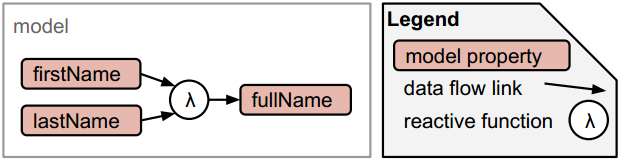
\includegraphics[width=\figureWidth]{figs/names.png}
  \caption [Full Name Reactive Model Example]{A basic reactive model that computes the full name whenever either the first name or last name changes. The reactive function is defined using the $when$ operator, therefore represents a node in a reactive data flow graph. }
  \label{fig:fullNameFlow}
\end{figure}

Lines 4 and 5 set a $when$ callback to log the full name whenever it changes. Lines 6 and 7 set the $firstName$ and $lastName$ properties on the $person$ model. This causes $fullName$ to be computed and set on the model. When $fullName$ is set, the callback that logs $fullName$ is invoked, causing the string \verb`"John Smith"` to be logged.

\section{Reactive Bar Chart} \label{reactiveBarChart}
Reactive models can serve as a foundation for interactive visualizations. Reactive models for multiple visualizations can be linked together at a higher level to form linked views. Interactive visualizations must respond to changes made by users such as resizing the display, changes in the data driving the visualization, changes in visualization configuration, and updates from other visualizations in a linked view context. This section introduces reactive visualization concepts through the example of a Bar Chart, then presents reusable reactive visualization components extracted from the Bar Chart.

A bar chart takes as input an array of data entries and a configuration that specifies the mapping from data attributes to the X and Y axes. It yields a dynamic bar chart graphic as output. The behavior desired for building the bar chart in response to changes in data and configuration fit perfectly within the framework of reactive models. As a first pass at constructing a reactive bar chart, the following reactive model properties are introduced:

\begin{itemize}
\item \verb`data` The input data table
\item \verb`xAttribute` The attribute used for the X scale (bar name)
\item \verb`yAttribute` The attribute used for the Y scale (bar height)
\end{itemize}

Using these three properties alone supports the essence of a bar chart, the plotting of bars and the labeling of axis tick marks. However, as attribute names are often cryptic and may not be the best labels for visualizations, two more model properties can be introduced that specify the text content of X and Y axis labels:

\begin{itemize}
\item \verb`xAxisLabel` The string displayed as the X axis label
\item \verb`yAxisLabel` The string displayed as the Y axis label
\end{itemize}

Bar charts and many other visualizations have an inner visualization rectangle in which visual marks are plotted. This inner rectangle lies within the outer rectangle containing the entire visualization, offset from the outer box by a specified margin. To integrate margin logic with reactive models, the following model properties are introduced:

\begin{itemize}
\item \verb`size` The size of the outer rectangle that contains the entire visualization, defined as an object with $width$ and $height$ properties in pixels.
\item \verb`margin` The margin object, having properties \verb`left`, \verb`right`, \verb`top` and \verb`bottom` in pixels, according to the D3 margin conventions \cite{d3conventionalmargins}.
\item \verb`width` The width of the inner visualization rectangle in pixels.
\item \verb`height` The height of the inner visualization rectangle in pixels.
\end{itemize}

The model properties defined this far support encapsulation of conventional D3 margins. A reactive function can be defined that updates $width$ and $height$ based on $size$ and $margin$. With the attributes present, scales can also be computed by reactive functions. The X scale depends on $data$, $xAttribute$, and $width$. The Y scale depends on $data$, $xAttribute$, and $height$. With the X and Y scales defined, the last remaining step is to compute the bars and axes from the data and scales. The complete reactive flow graph for a bar chart is shown in figure \ref{fig:barChartFlow}.

\begin{figure}
  \centering
  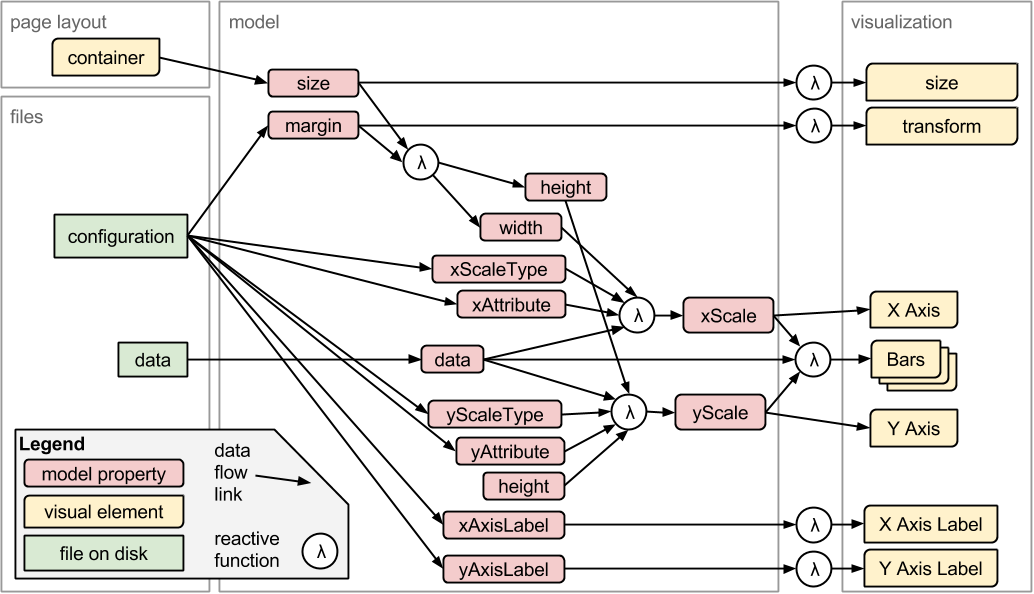
\includegraphics[width=\figureWidth]{figs/barChartFlow.png}
  \caption [Reactive Bar Chart Flow]{The data flow graph for a reactive bar chart based on \emph{reactive models}.}
  \label{fig:barChartFlow}
\end{figure}

\section{Reusable Reactive Flows}
Consider the following visualization techniques:
\begin{itemize}
\item Bar Chart
\item Scatter Plot
\item Line Chart
\item Stacked Area Chart
\end{itemize}

These visualizations share many underlying primitives such as scales, axes, and margins. The D3 Open Source project provides high quality generalized solutions for these and many more visualization primitives \cite{d3}. These visualization primitives and their computational dependency structure can be encapsulated by reactive flow graphs. Interactive forms of these visualizations also share interaction techniques for selecting visual marks such as rectangular brushing, hovering, clicking, panning, and zooming. Table \ref{table_components} lists reusable reactive flows common to many visualizations.

Other visualization techniques that may also be implemented using reactive models as a foundation include:

\begin{itemize}
\item Parallel Coordinates
\item Choropleth Map
\item Table
\item Box Plot
\end{itemize}

\newcommand{\diagramWidth}{1.9in}
\newcommand{\diagramScale}{0.4}
\newcommand{\descriptionWidth}{2.8in}
\newcommand{\descriptionPadding}{\vspace{.3\baselineskip}}

\begin{table*}
  \caption{Reusable flows for reactive visualization.}
  \centering
  \label{table_components}
  \begin{tabular}{ | c | c | c |}
    \hline
    \textbf{Component}
      & \textbf{Diagram}
      & \textbf{Description} \\ \hline
    margin
      & \parbox[c]{\diagramWidth}{\centering 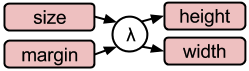
\includegraphics[scale=\diagramScale]{figs/margin.png}}
      & \parbox[c]{\descriptionWidth}{\descriptionPadding Computes the size of the inner visualization rectangle based on the container size (which may change when the user resizes the visualization) and the configured margin. \descriptionPadding}
      \\ \hline
    xScale
      & \parbox[c]{\diagramWidth}{\centering 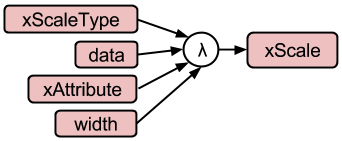
\includegraphics[scale=\diagramScale]{figs/xScale.png}}
      & \parbox[c]{\descriptionWidth}{ \descriptionPadding Computes the X scale. The domain is computed from the input data by evaluating the X attribute bounds. The range is computed from the inner visualization width. \descriptionPadding }
      \\ \hline
    xAxis
      & \parbox[c]{\diagramWidth}{\centering 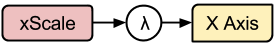
\includegraphics[scale=\diagramScale]{figs/xAxis.png}}
      & \parbox[c]{\descriptionWidth}{ \descriptionPadding Renders the X Axis (line, tick marks and labels) from the X scale \descriptionPadding.}
      \\ \hline
    xAxisLabel
      & \parbox[c]{\diagramWidth}{\centering 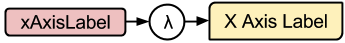
\includegraphics[scale=\diagramScale]{figs/xAxisLabel.png}}
      & \parbox[c]{\descriptionWidth}{ \descriptionPadding Renders the text label for the X Axis \descriptionPadding.}
      \\ \hline
    yScale
      & \parbox[c]{\diagramWidth}{\centering 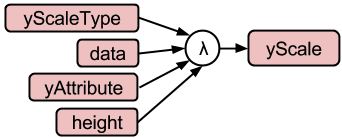
\includegraphics[scale=\diagramScale]{figs/yScale.png}}
      & \parbox[c]{\descriptionWidth}{ \descriptionPadding Computes the Y scale. The domain is computed from the input data by evaluating the Y attribute bounds. The range is computed from the inner visualization width. \descriptionPadding }
      \\ \hline
    yAxis
      & \parbox[c]{\diagramWidth}{\centering 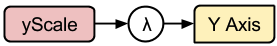
\includegraphics[scale=\diagramScale]{figs/yAxis.png}}
      & \parbox[c]{\descriptionWidth}{ \descriptionPadding Renders the Y Axis (line, tick marks and labels) from the Y scale \descriptionPadding.}
      \\ \hline
    yAxisLabel
      & \parbox[c]{\diagramWidth}{\centering 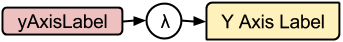
\includegraphics[scale=\diagramScale]{figs/yAxisLabel.png}}
      & \parbox[c]{\descriptionWidth}{ \descriptionPadding Renders the text label for the Y Axis \descriptionPadding.}
      \\ \hline
    colorScale
      & \parbox[c]{\diagramWidth}{\centering 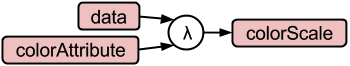
\includegraphics[scale=\diagramScale]{figs/colorScale.png}}
      & \parbox[c]{\descriptionWidth}{ \descriptionPadding Computes the color scale. The domain is computed from the input data by evaluating the set of unique values found in the color attribute. \descriptionPadding }
      \\ \hline
  \end{tabular}
\end{table*}

Property names serve as the common elements between components. Property names used in one or more components not introduced in the Bar Chart include:

\begin{itemize}
\item \verb1xScale1 The scale (domain and range) for the X axis.
\item \verb1xScaleType1 \verb1xScale1 qualifier: linear, logarithmic, or ordinal.
\item \verb1xAxis1 The visible X axis (tick marks and labels).

\item \verb1yScale1 The scale (domain and range) for the Y axis
\item \verb1yScaleType1 \verb1yScale1 qualifier: linear, logarithmic, or ordinal.
\item \verb1yAxis1 The visible Y axis (tick marks and labels).

\item \verb1colorAttribute1 The scale used to determine color of visual marks.
\item \verb1colorScale1 The scale used to determine color of marks.
\end{itemize}

Table \ref{table_components} lists components that can be combined to easily generate a foundation for a variety of interactive visualizations. These components encapsulate reusable reactive flows that implement the primitives necessary for interactive visualizations. Figure \ref{fig:barChartFlow} showed how several of these components can be assembled to create a general-purpose reactive bar chart. This bar chart flow represents a template for other visualizations, such as scatter plots. In fact, the only things that need to be changed in the bar chart flow to make it a scatter plot are (1) the X axis must be made quantitative, and (2) dots should be plotted rather than bars. Similarly, only the visual marks must be modified to change a scatter plot to a line chart, shown in figure \ref{fig:lineChart}.

\begin{figure}
  \centering
  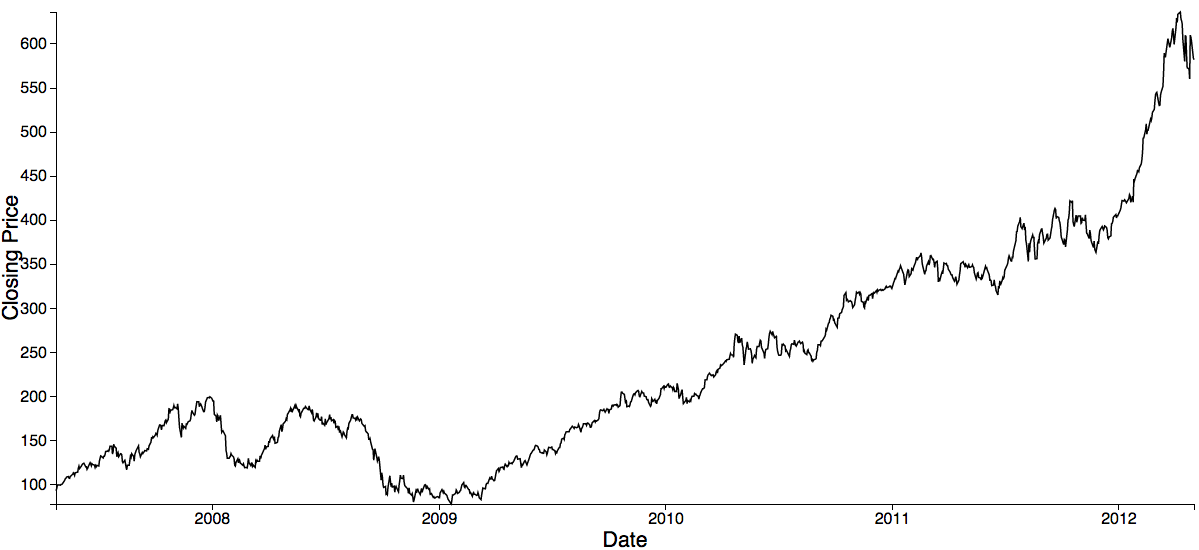
\includegraphics[width=\figureWidth]{figs/lineChart.png}
  \caption [Reactive Line Chart]{A line chart that shares scale and axis flows with scatter plots and bar charts.}
  \label{fig:lineChart}
\end{figure}

Interactive user interface components can be linked with any reactive model property. This makes it straightforward to add interactivity to reactive visualizations using conventional user interface elements such as dropdown menus, check boxes, sliders, and color pickers. For example, the X and Y attributes used by the scatter plot in figure \ref{fig:configurableScatter} can be made configurable using dropdown menus.

\begin{figure}
  \centering
  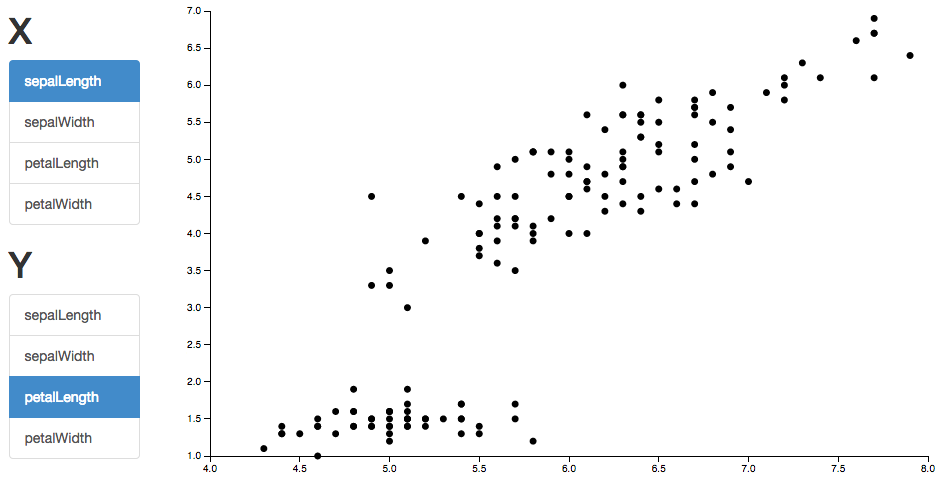
\includegraphics[width=\figureWidth]{figs/configurableScatter.png}
  \caption [Configurable Scatter Plot]{A scatter plot where X and Y attributes are selectable via Bootstrap List Group user interface elements.}
  \label{fig:configurableScatter}
\end{figure}
% and associated flow diagram.

% TODO include scatter plot flow diagram
% TODO make scatter plot flow diagram in Google Docs
% based on bar chart diagram.

% TODO automatically generate bar chart and scatter plot diagrams
\section{Linked Views}

Composing reactive visualizations from reusable flows yields reusable and composable interactive visualizations. Interactions such as brushing can be linked to the reactive model of the visualization instance. In the case of brushing, a model property \verb`brushedIntervals` contains the currently brushed intervals. This object stores the $(min, max)$ values for each attribute brushed. The updating brushed intervals can be used to as input to a filter operation that excludes data entries outside the brushed intervals. The output from the filter operator can be routed as input to another visualization. Figure \ref{fig:linkedViews} shows an example of linked views using this approach.

Figure \ref{fig:linkedViewsFlow} shows the overall flow of the linked scatter plot and bar chart. The brushing interaction sets a property on the reactive scatter plot called \verb1selectedData1. A reactive function that aggregates the selected data by Iris species links the selected data to the input data of the bar chart. Whenever the user brushes to select a new set of records in the scatter plot, the bar chart updates immediately to show only the selected data.

One advantage of reusable reactive flows is that when improvements are be made to a generalized feature, many visualizations manifest the improvement. For example, consider the X and Y axes used for many visualizations such as scatter plot and bar chart. The original D3 example that was drawn from to implement the axes had placed the axis labels inside the inner visualization rectangle. This had the unfortunate consequence that sometimes the label was occluded by marks within the visualization. To solve this issue, the axes were modified such that labels are placed outside the visualization area, are larger than tick mark labels, and are centered with respect to the axes. Figure \ref{fig:linkedViewsNew} shows the effect of the axis label improvement, which appears both in the scatter plot and bar chart.

\begin{figure}
  \centering
  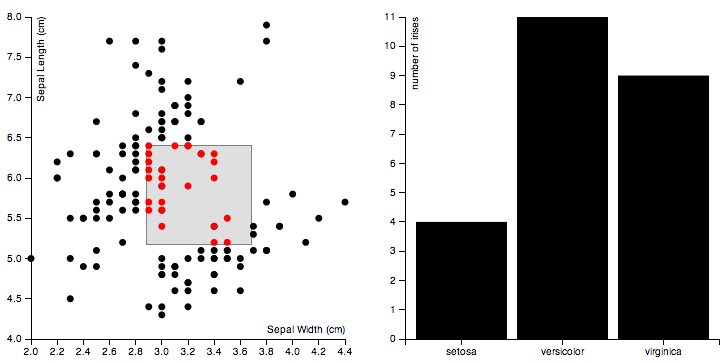
\includegraphics[width=\figureWidth]{figs/linkedViews.png}
  \caption [Linked Scatter Plot and Bar Chart]{A visualization of the Iris data set \cite{anderson1935irises} using linked views, powered by reactive visualization components. Brushing to select records in the scatter plot causes the selected data to be aggregated and displayed in the bar chart.}
  \label{fig:linkedViews}
\end{figure}

\begin{figure}
  \centering
  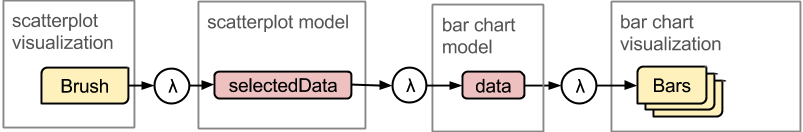
\includegraphics[width=\figureWidth]{figs/linkedViewsFlow.png}
  \caption [Linked Views Flow]{The (simplified) data flow graph for the linked scatter plot and bar chart example shown in figure \ref{fig:linkedViews}.}
  \label{fig:linkedViewsFlow}
\end{figure}

% TODO automatically generate linked view diagram

% TODO consider lazily evaluated model properties. Motivation: compute selected records from brush in scatter plot only when necessary.


\begin{figure}
  \centering
  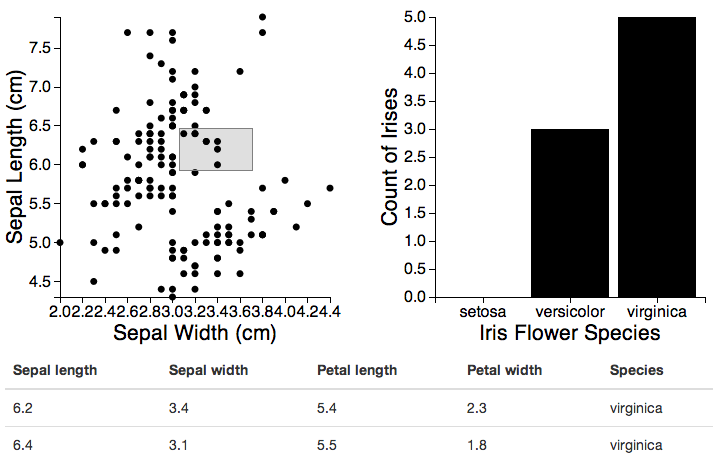
\includegraphics[width=\figureWidth]{figs/linkedViewsNew.png}
  \caption [Improved Linked Bar Chart, Scatter Plot and Table]{An improved version of the linked bar chart and scatter plot example. When changes are made in reusable components such as axes, the improvement is inherited by many reusable visualizations. This version also integrates with the reusable Bootstrap table component, showing the brushed selection in the table.}
  \label{fig:linkedViewsNew}
\end{figure}

\section{Summary}
This chapter introduced a novel way to combine elements of functional reactive programming with the Model View Controller (MVC) paradigm to create reactive models. Reactive models allow developers to specify data dependency graphs declaratively. This kind of abstraction is well suited for developing interactive visualizations because it drastically simplifies management of complex data flows and update patterns.

A collection of reusable reactive flows for interactive visualization was also introduced. These reactive flows encapsulate visualization primitives such as margins, scales, and axes. These flows were used as building blocks to generate a reusable bar chart, scatter plot and timeline. Visualizations with multiple linked views can be developed from these reusable visualization components in a straightforward manner .

\section{Future Work}
Future directions for this work will focus on developing a full catalog of reusable visualization components, coupling the data to currently available public data sources, visualization-centric user interfaces, and collaboration.

So far, the reactive visualization approach has been applied only to several visualization techniques. However, the following visualization techniques can also be supported:
\begin{itemize}
\item Color Legend
\item Pie Chart
\item Choropleth Map
\item Parallel Coordinates
\item Heatmap
\item Stacked Bar Chart
\item Stacked Area Chart
\item Streamgraph
\item TreeMap
\item Force Directed Graph Layout
\end{itemize}

Additionally, reusable components for the following interaction techniques can be encapsulated independently of any specific visualization technique using reactive models:
\begin{itemize}
\item Brushing - Dragging to define a selection region interactively.
\item Picking - Selecting a single visual mark by clicking or tapping on it.
\item Details-on-demand - A pattern of linked view composition in which an overview visualization can be used as navigation for a detailed view. This is a fundamental concept in interactive information visualization \cite{shneiderman1996eyes}.
\end{itemize}

A user interface for quickly assembling reusable components together based on graph drawing can also be developed. This user interface would show the data dependency diagrams similar to figure \ref{fig:barChartFlow}, but they would be dynamic and editable. Another direction for future research is integrating external user interface components such as traditional list selections, drop down menus, and radio buttons. One example of this concept is shown in figure \ref{fig:table}, which shows how reactive models can provide reactive HTML tables that can be linked with interactive visualizations. This would help in constructing intuitive user interfaces for manipulating the configuration of visualizations.

\begin{figure}
  \centering
  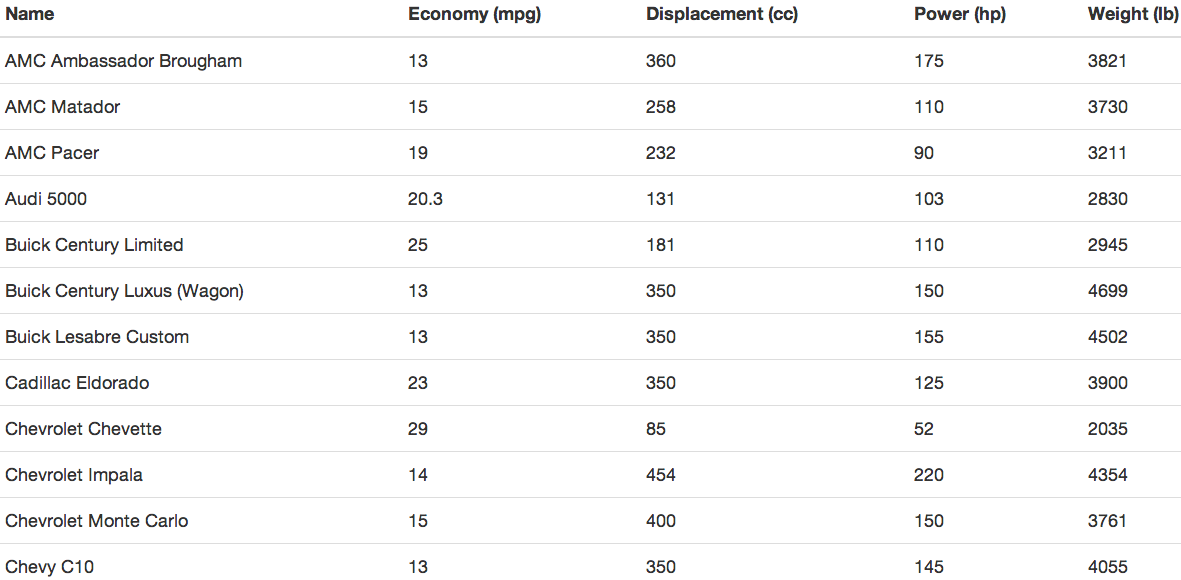
\includegraphics[width=\figureWidth]{figs/table.png}
  \caption [Reactive Table Visualization]{A visualization of the Cars data set \cite{hauser2002angular} by a reactive component that renders an HTML table style using Twitter Bootstrap \cite{lerner2012forge}.}
  \label{fig:table}
\end{figure}



\chapter{Collaborative Visual Data Exploration}
The utility of interactive visualizations depends on the ability of users to create them. Typically, data scientists or analysts work in teams. Contributions are made from every person on the team, and then the team must present their findings in a non-exploratory context. Sometimes it is useful to be able to show the path of exploration that the team has taken, using some kind of history model. This chapter presents an approach to enabling all of the above features, leveraging reactive models.

\section{Related Work}
Several projects have focused explicitly on visualization of public data on the Web. ManyEyes was an experiment in scaling the audience for visualizations by empowering users to create visualizations of their own data \cite{viegas2007manyeyes}. ManyEyes provided a fixed set of pre-packaged visualization tools and allowed users to visualize their own data tables using the provided visualizations. GapMinder is a project aimed at exposing public data (primarily the United Nations Millenium Development Goals Indicators) using visualization \cite{rosling2005new}. GapMinder includes an animated scatter plot with an interactive time slider, a line chart showing statistics over time, and a world map (see figure \ref{fig:gapminder}). The Google Public Data Explorer provides a visual interface to selected public data sets similar to GapMinder, but it does not make the data available to users in machine-readable form \cite{googlePublicDataExplorer}.

\begin{figure}[h!]
  \centering
  \includegraphics[width=\figureWidth]{figs/gapminder.jpg}
  \caption[GapMinder and Hans Rosling.]
   {GapMinder, a public data visualization tool based on an animated scatter plot, timeline, and map. Here, Professor Hans Rosling, the creator of GapMinder, is shown gesturing the motion of the plot while presenting the visualization.}
  \label{fig:gapminder}
\end{figure}
\pagebreak

Many data visualization and analysis tools have been developed with collaboration in mind. Tableau Server has collaboration features such as sharing visualizations, commenting on visualizations, embedding visualizations in Web pages, and sharing filtered data. The OpenChorus project supports annotation and sharing of data sources using a variety of database technologies including SQL, Hadoop (HDFS), Oracle, and Greenplum \cite{openChorus}. Foundational collaboration technologies include Operational Transform for synchronous collaboration such as Google Docs \cite{sun1998operational} and revision control systems for asynchronous collaboration such as GitHub \cite{o2009making, dabbish2012social}.

\section{Application State Model}
An application typically consists of instantiations of many reusable components. For example, an AngularJS application instantiates reusable components encapsulated as Angular directives, and a BackboneJS application instantiates Views for specific Models.

Interactive visualizations with multiple linked views share common patterns, including layout based on nested boxes and view linkage based on flows between interaction output, data transformations, and visualization input. This configuration can be expressed as a set of reactive models. Some models, such as the layout and linkages, must be able to access other models in the system and change their properties (e.g., the bounding box for layout and the selected elements for linked views). A simple structure based on named models can accommodate the above needs.

Our application state structure consists of \emph{components}, each of which has:
\begin{itemize}
\item \emph{alias} The string identifier for the component.
\item \emph{module} The string that defines which module to instantiate.
\item \emph{model} A collection of serialized model properties.
\end{itemize}

This structure can be serialized using JSON \cite{crockford2006application}. The overall application state configuration is an object whose keys are component aliases, and whose values are component objects. Each component object contains key-value pairs representing its serialized model state. Each component also has a value for the \verb1module1 property that determines which module is invoked to instantiate the component at runtime. Figure \ref{fig:dashboardLayout} shows an example of a configuration that instantiates simple components into a nested box layout. This layout technique is one of the foundations for assembling linked views. Any reusable visualization can be placed into a box in the layout, then linked with other visualizations within the same layout. Figure \ref{fig:prototype} shows an example nested box layout that includes visualizations.

\begin{figure}
  \centering
  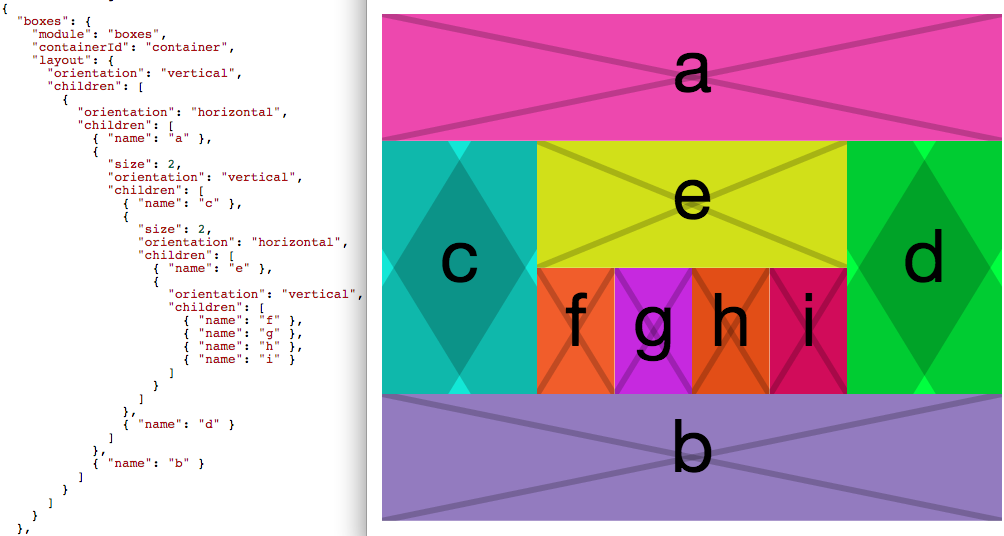
\includegraphics[width=\figureWidth]{figs/boxes.png}
  \caption [Nested Box Layout Configuration]{An example configuration that defines a nested box layout. }
  \label{fig:dashboardLayout}
\end{figure}

\begin{figure}
  \centering
  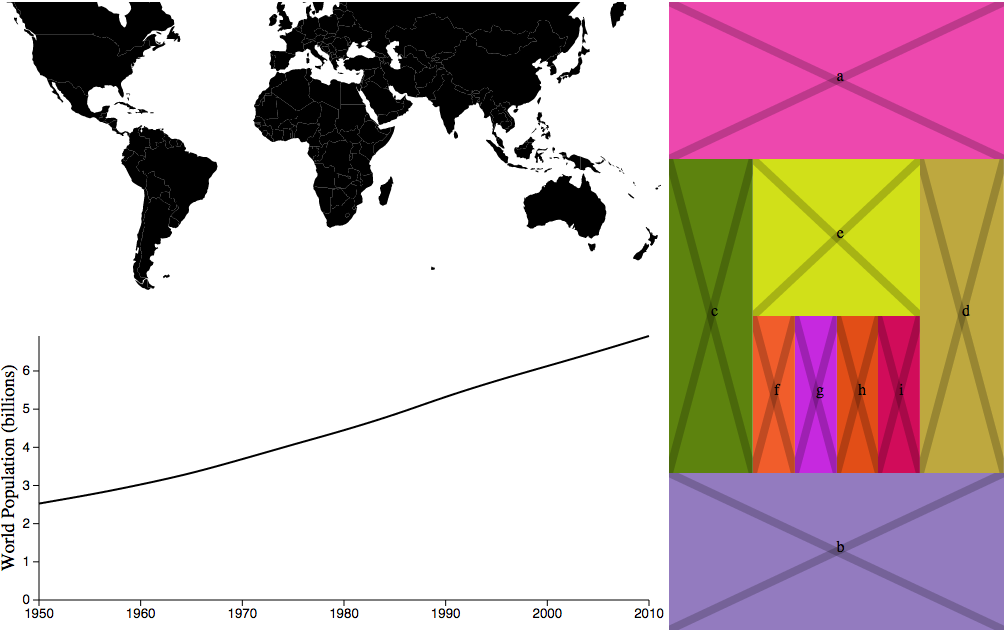
\includegraphics[width=\figureWidth]{figs/prototype.png}
  \caption [Nested Boxes with Visualizations]{An example configuration that defines a nested box layout including line chart and map visualizations. }
  \label{fig:prototype}
\end{figure}

\section{Runtime Engine}
The application state model addresses the configuration and serialization structure of the application state. A runtime model is necessary to transform serialized application state models into a running system. The runtime engine performs this transformation as follows:

\begin{itemize}
\item The runtime engine module loader is instantiated. This process defines a mapping from module names to constructor functions that instantiate the components, returning reactive models.
\item The \verb`module` property of each component in the application state configuration is used to instantiate each component.
\item The runtime engine maintains a dictionary whose keys are component aliases and whose values are instantiated components.
\item Instantiated components can request references to other instantiated components from the runtime. This operation must be asynchronous to account for dynamic module loading.
\end{itemize}

As an example, consider the flow of instantiation for the application state shown in figure \ref{fig:dashboardLayout}. The runtime uses the \verb1module1 property on each component to fetch and invoke its constructor module. The \verb`boxes` module computes the nested box layout. The computed nested box layout is used for dynamically positioning and sizing the interactive visual components.

The first prototype of the interactively configurable runtime engine was developed during a summer internship at Rapid7, a cybersecurity company, to create an interactive visualization dashboard with multiple linked views for analyzing corporate login activity. Technologies used for visualization included D3.js, a visualization framework that uses SVG, and Leaflet.js, a framework for geographic maps. The map showed where users have logged into the network, aggregated geographically using the Leaflet MarkerCluster plugin and visualized using D3's Pie Chart layout. Black represented successful logins and blue represented failed logins. This industry application of our dashboard layout framework demonstrates its capability to define dashboards with multiple linked views. The resulting visualization dashboard is shown in figure \ref{fig:ingressDash}.

\begin{figure}
  \centering
  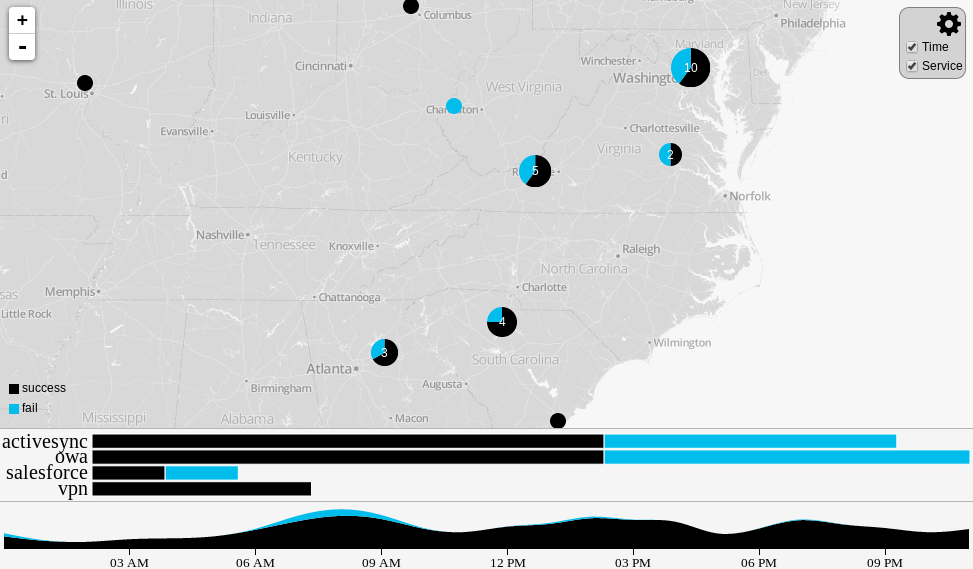
\includegraphics[width=\figureWidth]{figs/mapDocs7.png}
  \caption[The Rapid7 Ingress Dashboard.]
   {This visualization dashboard shows corporate login data and is integrated into the Rapid7 product called UserInsight.}
  \label{fig:ingressDash}
\end{figure}

\begin{figure}
  \centering
  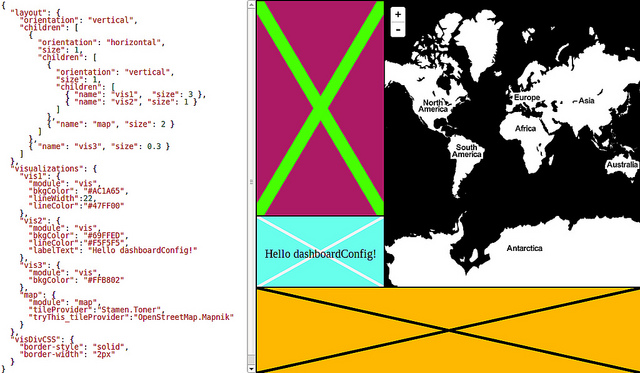
\includegraphics[width=\figureWidth]{figs/dashboardScaffold.png}
  \caption[Dashboard Scaffold Configuration Editor.]
   {The dashboard scaffold prototype, showing an interactive text-based configuration editor on the left, and a sample dashboard on the right. This shows how Leaflet-based maps can be integrated with D3 visualizations using the proposed configuration framework.}
  \label{fig:ingressDash}
\end{figure}

\section{Changing State}
When the application state configuration changes, the runtime components must be updated accordingly. Consider the scenario of a user manually editing the application state configuration using a text editor. Every time the user changes the configuration, the system must update the runtime to reflect the new configuration. A na\"{\i}ve approach to this problem is to tear down and re-instantiate the entire runtime whenever the configuration changes. This approach, while functionally correct, does an extraordinary amount of unnecessary work. A more efficient solution would employ a strategy in which only the changes in configuration are propagated through the runtime, while unchanged configuration parameters need not have any effect on the runtime.

All application state configuration updates can be expressed as a series of the following operations:
\begin{itemize}
\item create(alias, module)
\item destroy(alias)
\item set(alias, property, value)
\item unset(alias, property)
\end{itemize}

In the context of a user manually updating the configuration at runtime, the difference between two configurations can be computed. The difference results in a structure that can be applied to the runtime essentially as a patch.

\section{Real-time Synchronization}
While Operational Transform algorithms address the general case of many-way synchronization for arbitrary text \cite{cormack1995counterexample}, if we have a simpler application state configuration structure, it is possible to implement simpler many-way synchronization algorithms. Our simple application state configuration difference structure provides an important primitive for real time configuration. The configuration difference objects computed locally can be broadcast to other clients and applied to remote runtimes to achieve real time many-way synchronization.

To implement real time synchronization, consider the application state and its changes as a directed graph $G = (V, E)$. Vertices in the graph represent application states, and each directed edge between nodes $u$ and $v$ represents a change in state. In a distributed environment with multiple clients, any client can originate a new state. The client that creates a new state provides the associated configuration difference object that can move any client runtime from state $u$ to state $v$ when applied.

Situations may arise in which the source state $u$ of a new state transition does not match the current runtime state. This occurs when two or more clients simultaneously originate conflicting state changes. The distributed synchronization algorithm must guarantee that no matter which order the conflicting state transitions arrive at the server, all clients must ultimately end up in the same state. This requirement can be implemented with simple algorithms that throw away some changes, or more complex algorithms that preserve every change.

Simple distributed synchronization algorithms can be developed that implement either ``first one wins'' or ``last one wins'' semantics. First one wins semantics means that the first of several conflicting state transitions that arrives at the server is accepted as the authoritative one and forced upon clients, causing the clients to roll back local conflicting changes. Last one wins semantics means that the last of several conflicting state transitions that arrives at the server is accepted as the authoritative one, causing the server to compute rollbacks and broadcast them to clients. Either way, clients experience loss of changes. In use cases with many concurrent users making changes simultaneously, these semantics would lead to frustrating user experiences, as users must perform their actions twice or more before they are accepted into the authoritative state.

%TODO include pseudocode and diagrams for first one wins and last one wins semantics

More complex algorithms that involve merging conflicting state transitions can address multiple concurrent changes. These algorithms must merge multiple configuration difference objects and generate a new state originating at the server. The server, with awareness of the states of each client, must send different transitions to each client such that each client ultimately is in the new state that originated from the server.

%TODO include pseudocode and diagrams for merge

\section{History Model}
Using the state machine model discussed, transitions can be annotated with an undo operation to enable history graph navigation. Each transition that occurs in the system adds a forward edge (a ``do'' operation) and a backward edge (an ``undo'' operation) to the history graph. Numerous algorithms exist for computing the shortest path in an arbitrary directed graph \cite{gallo1988shortest}. A shortest path algorithm such as Dijkstra's can be used to compute the sequence of configuration difference objects to apply to a runtime in order to transition the system from any state to any other state.

\section{Integration with Web Technologies}
To build interactive visualizations for the Web using reactive models, there must be a clearly defined way to interface between reactive models and Web graphics technologies. The primary Web graphics technologies are Canvas and SVG (Scalable Vector Graphics). The Canvas element provides an additional API called WebGL that supports hardware accelerated graphics. The goal of integrating reactive models with Web graphics technologies is to build reusable interactive graphics modules. The modules can be instantiated and linked with specific data to create interactive visualizations.

Instantiations of reusable interactive graphics components in general function in conjunction with a DOM element. Therefore, one way to accommodate any Web technology is to design an API in which a module constructor function creates a DOM element that contains its visual representation. Cascading Style Sheets (CSS) can then be used to position the DOM element. This approach effectively unifies Canvas, WebGL, and SVG, and allows interactive graphics modules authored using different APIs to function together on a single page.



\chapter{The Universal Data Cube}
Consider the question ``Is there a correlation between the population of a country and its Gross Domestic Product (GDP)?''. The data for population and GDP can only be obtained independently from different sources. Suppose each data set is a relation. To apply visualization or analysis techniques to the data, the two relations must first be joined such that each row in the resulting relation represents a country and contains values for both population and GDP.

Integrating data from a variety of independent sources makes the data more useful, informative, and valuable for visualization and analysis tasks. Existing data integration and multidimensional analysis approaches typically target relational data sources. The data cube concept from the area of Online Analytical Processing (OLAP) is suitable for modeling statistical data sets. These approaches do not readily support integration of pre-computed data cubes, which is applicable for primarily scientific and social data analysis and visualization.

There is immense potential value in data that is not being realized. While publicly available data sets for just about any topic are published on the Web, it is difficult to realize their full value in practice because they exist in many different formats and vocabularies. The heterogeneity of these formats and vocabularies also makes it difficult to combine and analyze these data sets, and hinders the development of general purpose visualization tools.

This chapter presents novel data structures and algorithms for data set representation, integration and querying based on the data cube concept. The proposed framework is called the Universal Data Cube (UDC). Using this approach, many data sources can be integrated together into a single data structure. General purpose data visualization and analysis tools can then operate by querying the integrated data structure. Figure \ref{fig:flow} shows the overall flow enabled by the UDC, from disparate data sets to general purpose interactive visualizations.

\begin{figure}
  \centering
  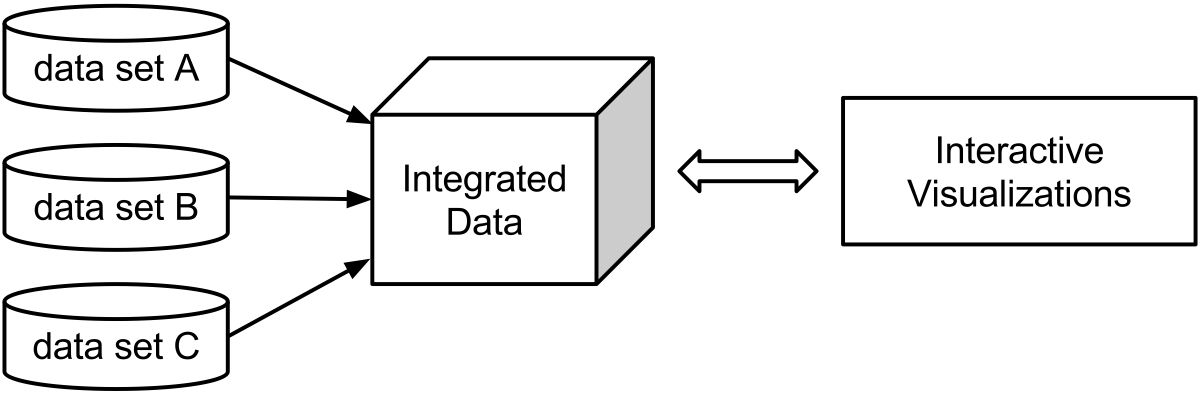
\includegraphics[width=\figureWidth]{figs/flow.png}
  \caption [Universal Data Cube Overview]{The overall context of the UDC as a technology for data integration for the purpose of interactive visualization. }
  \label{fig:flow}
\end{figure}

\section{Related Work}
Existing approaches to representing, visualizing, and analyzing are vast. The relational model is the foundation of relational databases. Data cubes are multidimensional aggregated relations suitable for visualization and analysis. The field of knowledge management is concerned with general data models representing vast collections of concepts and facts. Data integration is an area focusing on techniques for combining data from many sources.

Relational database systems provide a mature data management solution and are widely adopted \cite{ramakrishnan2000database}. Relational algebra is the theoretical underpinning of relational databases \cite{clifford1985algebra}. Perhaps the most familiar data representation system today is the spreadsheet, which is capable of representing relations as well as complex operations across data values \cite{eick2000visualizing}. Many organizations use spreadsheets, employing Microsoft Excel, Google Docs, or other tools to manage data or make data available. For example, the United Nations Department of Economic and Social Affairs provides their population statistics in Excel format (see figure \ref{fig:unPopExcel}).

The term ``data cube'' was originally introduced as a relational operator generalizing group-by, cross-tab, and sub-totals \cite{gray1997data}. The data cube operator produces relations containing aggregated values from other relations. Data warehouse systems are typically built on the relational model and are augmented by data cubes, also known as OLAP (OnLine Analytical Processing) cubes, for reporting and analysis \cite{codd1993providing}. The term OLAP stands in contrast to OLTP (OnLine Transaction Processing), which is the part of the data warehouse system that ingests and stores data at the level of individual transactions or events. After the ETL (Extract, Transform and Load) phase of the data warehouse flow, the data is analyzed by computing a data cube from the transactional data.

Data cubes contain summaries of the collection of facts stored in a relational database \cite{chaudhuri1997overview}. For example, a data cube may contain how much profit was made from month to month subdivided by product category, while the relational database may contain the information associated with each individual transaction. Because data cubes provide a higher level of abstraction, they are a widely used method of data abstraction for supporting visualization and analysis tasks. Kimball pioneered the area of ``Dimensional Modeling,'' which concerns constructing data warehouse schemas amenable to OLAP-based analysis \cite{kimball1998data}. Data cubes have been implemented in a variety of different systems, so effort has been made to discover unified conceptual or mathematical models that can characterize many implementations \cite{datta1999cube, vassiliadis1999survey, vassiliadis1998modeling, li1996data, agrawal1997modeling, gyssens1997foundation, blaschka1998finding}.

The data cube concept and structure can be used to model existing data as well. Publicly available data sets (often termed ``statistical data'') may be considered as pre-computed data cubes if they contain aggregated measures (also called ``indicators,'' ``metrics,'' or ``statistics'') across time, geographic space, and other dimensions such as gender, age range, ethnicity, religion, or industry sector.

Existing OLAP technologies assume that the data cubes will be computed from a relational source. They are not designed to handle integration of pre-computed data cubes that may use inconsistent identifiers for common dimensions and measures between multiple data sets. Therefore, the application of the data cube concept to integration and visualization of many pre-computed data cubes, while theoretically plausible, requires the development of novel data structures and algorithms that extend the data cube model to handle integration of pre-computed data cubes that may use inconsistent identifiers for common dimensions and measures. With this approach, it is possible to model many data sets using their shared dimensions and measures. This enables integration of many data sets into a single structure suitable for visualization and analysis.

The Semantic Web is a vision of a ``Web of Data'' coexisting with the World Wide Web \cite{berners2001semantic}. The basis of the Semantic Web is the Resource Description Framework (RDF) data model, which represents a graph of data in the form of $(subject, predicate, object)$ triples. The Semantic Web vision has evolved into the concept of Linked Data, which refers to data that is available as RDF and made available according to common conventions \cite{bizer2009linked, bizer2007publish}. Any data that can be represented using a relational database can also be represented using RDF \cite{bizer2006d2r}. The SPARQL query language for RDF can be used to query and integrate data from multiple sources \cite{quilitz2008querying}. Lopez et al.\ developed an information management system for integrating and analyzing heterogeneous information sources characterizing urban areas \cite{lopez2012queriocity}. The Semantic Web technology stack contains a method for declaring when different identifiers refer to the same entity and processing queries appropriately to integrate data \cite{halpin2010owl, ding2010sameas}. While the Semantic Web provides a compelling vision, its adoption is not as widespread as one might expect \cite{lytras2008semantic}.

The RDF Data Cube Vocabulary is capable of representing data cubes using Semantic Web technologies \cite{rdfdatacube}. The intention of the RDF Data Cube Vocabulary is to provide a common representation and interchange format for statistical data. The RDF Data Cube Vocabulary draws from a previous effort called the Statistical Data and Metadata eXchange (SDMX) initiative that was launched in 2001 by seven organizations working on statistics at the international level \cite{cyganiak2010semantic}. The primary challenges faced when using the RDF Data Cube Vocabulary include transforming to and from well known formats and data models. Salas et al.\ discussed how data can be transformed from existing OLAP systems or flat files into RDF using the Data Cube Vocabulary and introduced a faceted visualization tool for RDF data cubes \cite{salas-icsc-2012}. K{\"a}mpgen et al.\ investigated how data represented using the RDF Data Cube Vocabulary can be transformed for analysis using traditional OLAP systems \cite{kampgen2011transforming}. Maali et al.\ proposed a pipeline for converting government data into high quality Linked Data utilizing the Data Cube Vocabulary \cite{maali2012publishing}.

The field of data integration offers many techniques for combining data from multiple sources based on the relational model \cite{doan2012principles} as well as from a theoretical perspective \cite{lenzerini2002data, halevy2006data, ziegler2004three}. Schema matching is the area of data integration that concerns semantic matching between the attributes of data tables from different sources \cite{rahm2001survey, fagin2003data}.

Schema matching may be performed manually, but it must be automated to scale to hundreds or thousands of different sources. Numerous approaches for automated schema matching have been proposed \cite{shvaiko2005survey, doan2001reconciling, kang2003schema, milo1998using, madhavan2001generic, doan2000learning}. Schema matching approaches aimed specifically at Web- and Ontology-based data integration have also been proposed \cite{he2003statistical, noy2004semantic, doan2005semantic, madhavan2007web, kalfoglou2003ontology, noy2009ontology, uschold2004ontologies, wache2001ontology, noy2003prompt, euzenat2007ontology}.

Data matching (also known as record linkage) is the area of data integration focusing on resolving different identifiers to the same real-world entity \cite{winkler1999state, winkler2006overview, koudas2006record, aizawa2005fast, gu2003record}. Record linkage has been applied extensively to public data \cite{jaro1995probabilistic, jaro1989advances, holman1999population}. Several tools have been introduced that aid users in data integration tasks via a graphical user interface \cite{christen2008febrl, kandel2011wrangler, elfeky2002tailor, gonzalez2010google}. Techniques from both of these areas must be applied to integrate data sets from multiple sources and use the proposed unified data model.

\section{Case Study: Causes of Death}
The Centers for Disease Control provides data on causes of death in the US over time. This data set was targeted for visualization as a case study in visualizing public data sets containing pre-aggregated data cubes. A natural way to visualize this data is as a stacked area chart, shown in figure \ref{fig:mortalityVisV2}. The table contained a hierarchy of diseases, and all but the top-level disease categories were removed manually. Selecting the subtree of causes of death to include in the visualization is one example of a task that would be automated with our data representation framework. Next, a JavaScript program was written that pivoted the table from a format where each column was a year to a format where each row is a year, making the table usable by D3.js. This table contained an entry for ``all causes,'' which was removed manually because it was not appropriate to include visualize.

The mortality data set was published in GitHub Pages using JavaScript Object Notation (JSON) \cite{crockford2006application} compatible with the structure accepted by D3 \cite{d3}. AMD (Asynchronous Module Definition) is a JavaScript pattern for publishing and consuming reusable modules across domains \cite{osmani2012learning}. The mortality data set was published as an AMD module containing JSON data rather than as a CSV or JSON file in order to circumvent the same-origin policy. This allows any Web page to consume the data set, not only pages within the same domain. This method of publishing was chosen because it is a simple way to publish data publicly with zero cost (as GitHub Pages is a free service for Open Source code), longevity, as GitHub is less likely to go offline in the future than a private server, and cross-domain availability (any page can load the module using an AMD loader such as \verb1require.js1). This method of publishing data is also developer-friendly, as most modern developers are familiar with GitHub.

The mortality stacked area visualization highlights several issues that must be addressed when using our proposed data representation framework. The causes of death extracted from the raw data are sometimes too long to use in the visualization as labels due to limited screen real estate. For example, ``Symptoms, signs, and abnormal clinical and laboratory findings, not elsewhere classified'' is too long to be placed next to its corresponding color in the legend of the visualization, and could be simplified to ``Unclassified conditions.'' In a data cube model, causes of death would be members in a dimension hierarchy. The labeling issue encountered in the mortality visualization indicates a need to support renaming of members for use as textual elements within visualizations. Since each label refers to a dimension member which may also be a generally well-known concept, the labels on the visualization could, for example, be links to the Wikipedia pages about the various causes of death, such as Cardiovascular Disease. In addition, there are 24 causes of death presented in this visualization using different colors, while the color scales provided by D3 and the color scale library ColorBrewer only support up to 20 colors. This issue indicates that it may be useful to be able to aggregate dimension members automatically as a new ``Other'' category in certain cases, or allow users to manually select only a subtree of a dimension hierarchy for visualization.

\begin{figure}[h!]
  \centering
  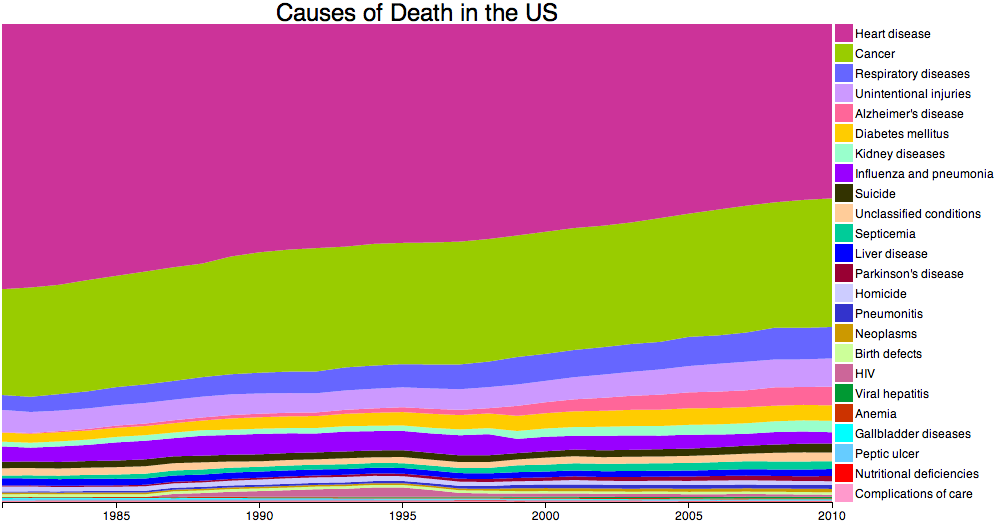
\includegraphics[width=\figureWidth]{figs/mortalityVisV2.png}
  \caption[CDC Mortality Visualization Version 2.]
   {A second pass at a stacked area visualization of Mortality data from the US Centers for Disease Control. This version has 25 hand-picked distinguishable colors, a color legend to spread out labels, and shortened labels in some cases.}
  \label{fig:mortalityVisV2}
\end{figure}

Figure \ref{fig:cardiovascularDiseaseRawTree} shows a sample of the raw data from which the hierarchy of causes of death must be gleaned. In this data, the hierarchy is encoded as an indented tree. Two different characters are used as indentation characters, ASCII codes 32 (space) and 65533 (unknown character). The level of indentation does not use a consistent number of indentation characters per indentation level. For example, the indentation level jumps from 0 to 4 to 7 to 10 to 13. We implemented an algorithm that parses the tree structure from an indented list and outputs the tree in the JSON structure compatible with D3.js hierarchical layouts. The JSON that the D3 Tree Layout algorithm expects is a tree data structure in which each node has a name and an array of child nodes. Leaf nodes may have additional quantitative properties to be visualized \cite{d3TreeLayout}.

Several D3 examples were drawn from to implement the cause of death tree visualization shown in figure \ref{fig:mortalityVisTree}, which uses the Reingold–Tilford ``tidy'' tree layout algorithm \cite{reingold1981tidier}. This visualization shows only the hierarchy of causes of death. No numerical values are associated with each node. Notice that the two causes of death that show the highest percentages in our stacked area visualization, Cancer and Cardiovascular Diseases, are the two nodes in the hierarchy that have the two largest subtrees of categorization.

The node-link tree visualization in figure \ref{fig:mortalityVisTree} demonstrates a visualization technique that can be applied to visualize dimension hierarchies in general. This implementation shows the structure of the hierarchy clearly, but has several drawbacks. Due to the size of the hierarchy, the inclusion of labels for all nodes necessitates small labels that are only legible at high resolution. When a hierarchy scales above certain thresholds of width and depth, this visualization becomes unwieldy, and labels must be truncated or omitted entirely. This is one example of the scalability issues that must be addressed when developing general-purpose visualization techniques.

\begin{figure}
  \centering
  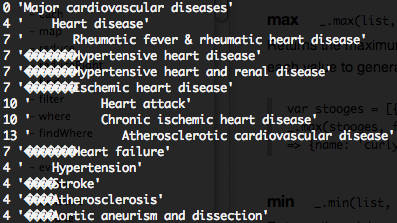
\includegraphics[width=\figureWidth]{figs/cardiovascularDiseaseRawTree.png}
  \caption[Cardiovascular disease raw tree.]
   {A portion of the raw data from the Centers for Disease Control encoding the hierarchy of causes of death. The number of indentation characters is shown on the left, and the content of the ``Cause'' field from the original CSV file is shown on the right in quotes. Note that there are two different indentation characters used, and the indentation level is not of a consistent multiple. This is one example of an unconventional format that must be parsed into a dimension hierarchy for use within our data representation framework.}
  \label{fig:cardiovascularDiseaseRawTree}
\end{figure}

\begin{figure}
  \centering
  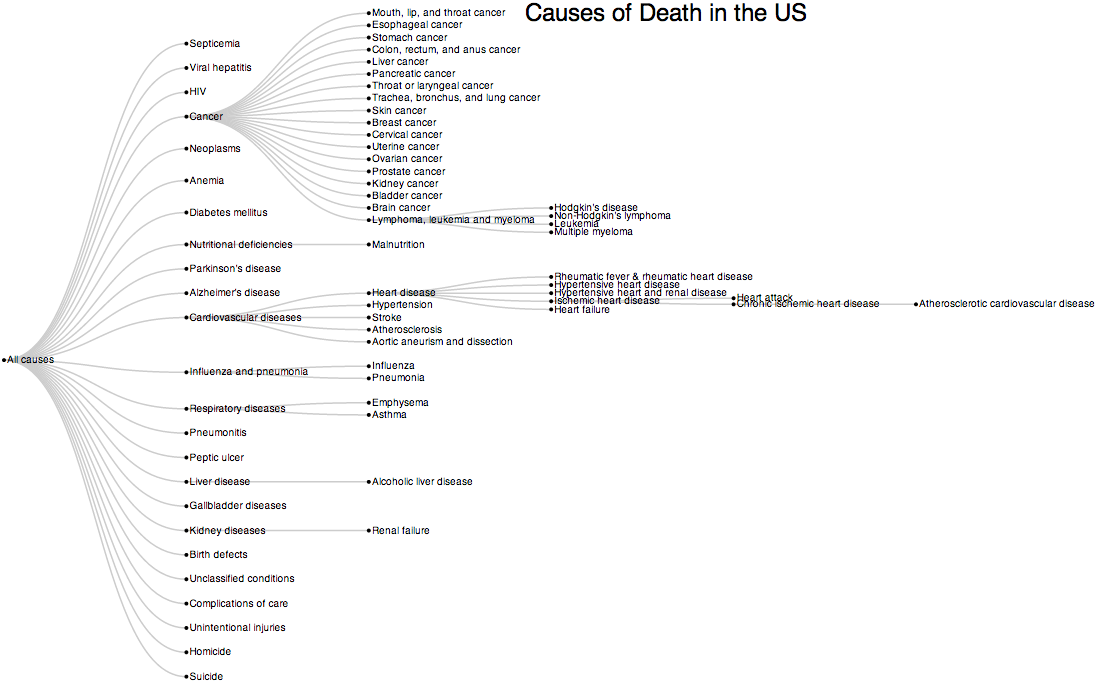
\includegraphics[width=\figureWidth]{figs/mortalityVisTree.png}
  \caption[Cause of Death Tree Visualization.]
   {A tree visualization of data from the Centers for Disease Control showing the hierarchy of causes of death. This is one example of a visualization that shows the structure of a dimension hierarchy.}
  \label{fig:mortalityVisTree}
\end{figure}

The pair of visualizations shown in figure \ref{fig:mortalityVisV4} is an example of a visualization dashboard with multiple linked views. The tree view shows a single level subtree. Black nodes have children, while white nodes do not. Clicking a black node causes the tree to drill down into the subtree with the clicked node as its root. When this interaction is executed, the stacked area visualization is recomputed to show the new set of disease causes that corresponds to the children of the newly selected node. In this way, the tree visualization provides interactions for drill down and roll up that define the slice of data shown in the stacked area chart.

\begin{figure}
  \centering
  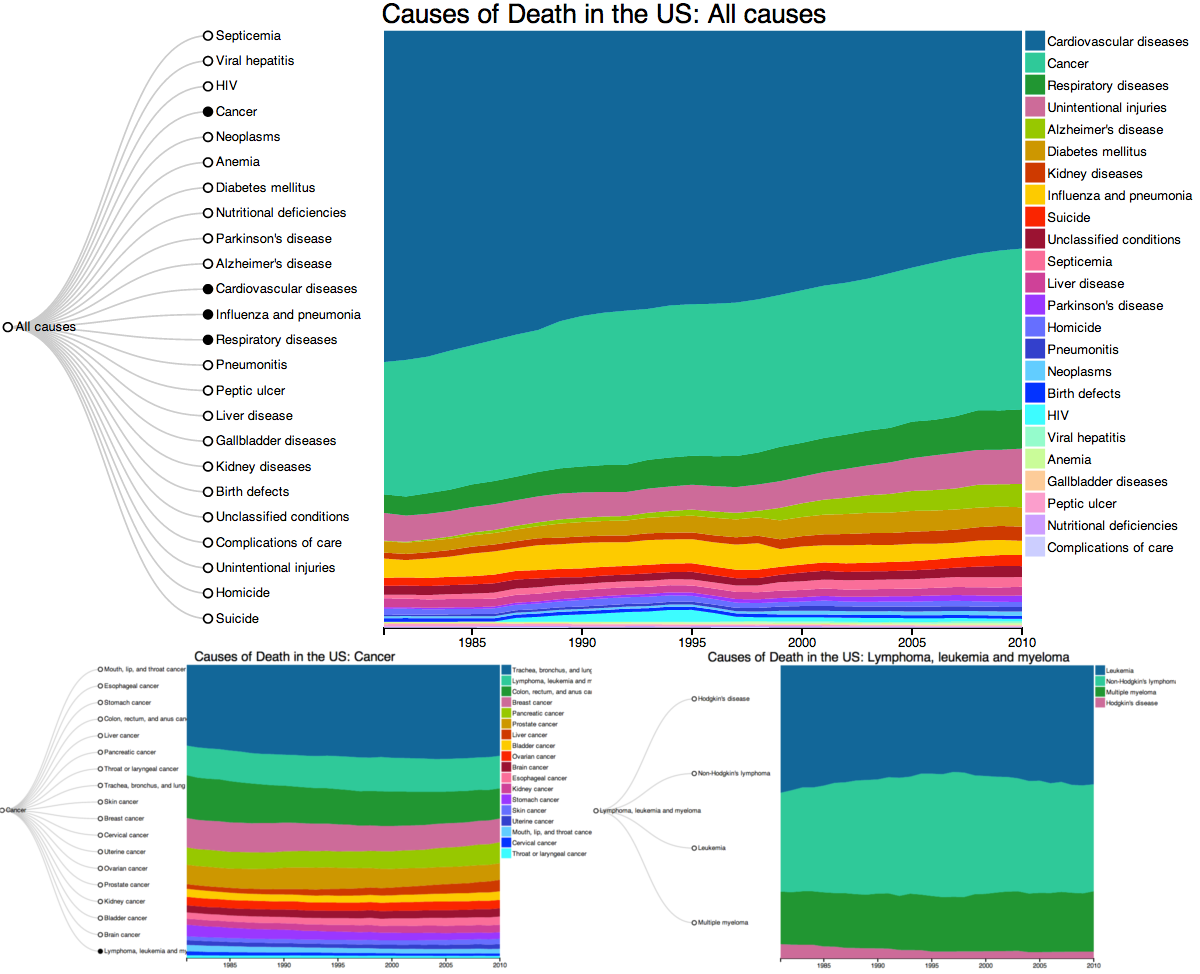
\includegraphics[width=\figureWidth]{figs/mortalityVisV4.png}
  \caption[CDC Mortality Visualization with Linked Views.]
   {Cause of death visualization with two linked views. Navigating up and down the hierarchy by clicking nodes changes the slice of data shown in the stacked area visualization. The top view shows the top-level causes of death. Clicking the ``Cancer'' node yields the view on the bottom left, which shows types of cancer in the stacked area visualization. Further drilling down to ``Lymphoma, leukemia and myeloma'' yields the view on the bottom right.}
  \label{fig:mortalityVisV4}
\end{figure}
\section{Data Set Representation}

In the sections that follow, capitalization denotes terms that have a concrete and well defined meaning within the UDC data structure. These terms include Data Set, Dimension, Member, Measure, Dimension Column, Measure Column, Cube Data Set, Concordance Data Set, Codelist, and Code. Each of these terms will be introduced one by one in terms of what role they play in the UDC data structure. Italicized terms are functions that perform the algorithms associated with data integration and querying. These algorithms operate in terms of the UDC data structure.

A Data Set is a relation with associated metadata that provides context for its interpretation. Tables \ref{table_gdp}, \ref{table_unPop} and \ref{table_concordance} are concrete examples of Data Sets, showing both their relations and metadata. The relation contains the core table of the Data Set. The metadata specifies the interpretation of the relation in terms of Dimensions and Measures. Columns in relations can be annotated in the metadata as either Dimension Columns or Measure Columns. A Dimension Column contains Codes from a single Codelist that refer to Members of a given Dimension. A Measure Column contains numbers representing values for a given Measure. A scaling factor can be associated with each Measure Column to account for varying scales for the same Measure across different Data Sets.

To integrate Data Sets together, we need two kinds of Data Sets, Cube Data Sets and Concordance Data Sets.

\begin{table}
  \caption{A Cube Data Set about Population.}
  \centering
  \label{table_unPop}
  \begin{tabular}{ | c | c | }
    \hline
    table & 
    \begin{tabular}{ | c | c | c | }
      \hline
      \textbf{countryCode} & \textbf{year}& \textbf{pop} \\ \hline
      356 & 1960 & 449595.489 \\ \hline
      356 & 2010 & 1205624.648 \\ \hline
      156 & 1960 & 650680.114 \\ \hline
      156 & 2010 & 1359821.465 \\ \hline
      840 & 1960 & 186361.893 \\ \hline
      840 & 2010 & 312247.116 \\ \hline
    \end{tabular}
    \\ \hline
    dimensions &
    \begin{tabular}{ | c | c | c |}
      \hline
      \textbf{column} & \textbf{dimension} & \textbf{codelist} \\ \hline
      countryCode & Space & UN M.49 \\ \hline
      year & Time & Year \\ \hline
    \end{tabular}
    \\ \hline
    measures & 
    \begin{tabular}{ | c | c | c |}
      \hline
      \textbf{column} & \textbf{measure} & \textbf{scale} \\ \hline
      pop & Population & 1,000 \\ \hline
    \end{tabular}
    \\ \hline
  \end{tabular}
\end{table}

\begin{table}
  \caption{A Cube Data Set about GDP.}
  \centering
  \label{table_gdp}
  \begin{tabular}{ | c | c | }
    \hline
    table & 
      \begin{tabular}{ | c | c | c | }
        \hline
        \textbf{countryCode} & \textbf{year} & \textbf{gdp} \\ \hline
        IND & 1960 & 37679274491.2745 \\ \hline
        IND & 2010 & 1708450861364.17 \\ \hline
        CHN & 1960 & 61377930682.0013 \\ \hline
        CHN & 2010 & 5930529470799.17 \\ \hline
        USA & 1960 & 520531181568 \\ \hline
        USA & 2010 & 14958300000000 \\ \hline
      \end{tabular}
    \\ \hline
    dimensions &
    \begin{tabular}{ | c | c | c |}
      \hline
      \textbf{column} & \textbf{dimension} & \textbf{codelist} \\ \hline
      countryCode & Space & ISO3 \\ \hline
      year & Time & Year \\ \hline
    \end{tabular}
    \\ \hline
    measures & 
    \begin{tabular}{ | c | c | c |}
      \hline
      \textbf{column} & \textbf{measure} & \textbf{scale} \\ \hline
      gdp & Gross Domestic Product & 1 \\ \hline
    \end{tabular}
    \\ \hline
  \end{tabular}
\end{table}

\begin{table}
  \caption{A Concordance Data Set linking equivalent terms used by different cubes referring to countries.}
  \centering
  \label{table_concordance}
  \begin{tabular}{ | c | c | }
    \hline
    table & 
    \begin{tabular}{ | c | c | c | }
      \hline
      \textbf{countryName} & \textbf{unCountryCode}& \textbf{alphaCode} \\ \hline
      India & 356 & IND \\ \hline
      China & 156 & CHN \\ \hline
      United States & 840 & USA \\ \hline
    \end{tabular}
    \\ \hline
    dimensions &
    \begin{tabular}{ | c | c | c |}
      \hline
      \textbf{column} & \textbf{dimension} & \textbf{codelist} \\ \hline
      countryName & Space & UN Geoname \\ \hline
      unCountryCode & Space & UN M.49 \\ \hline
      alphaCode & Space & ISO3 \\ \hline
    \end{tabular}
    \\ \hline
  \end{tabular}
\end{table}

A Cube Data Set contains a relation that represents a data cube using a star schema. Certain columns represent categorical Dimensions, while others represent quantitative Measures. Dimensions are sets of distinct entities that may be unordered, ordered, or hierarchical. Each distinct entity of a Dimension is called a Member. A row in the relation of a Cube Data Set represents a unique set of Members, one from each Dimension of the Cube Data Set, in its Dimension Columns. The unique set of Members represented in each row is called a Cell, which acts like an address in the data cube. Measures are aggregated quantitative properties that can be assigned to Cells in the Measure Columns of the relation. A Cube Data Set contains a set of Observations that draw from a common set of Dimensions and Measures. An Observation links a Cell with concrete values for each Measure. Each complete row of the relation represents a single Observation. Many Cubes can reference the same Dimensions, Members, Cells, and Measures, whereas each Observation belongs to exactly one Cube. Table \ref{table_concepts} provides examples for each of the concepts introduced.

\begin{landscape}
  \begin{table*}
    \caption{Examples for UDC Concepts.}
    \small
    \centering
    \label{table_concepts}
    \begin{tabular}{ | c | c | c |}
      \hline
      \textbf{Concept} & \textbf{Example(s)} & \textbf{Description} \\ \hline
      Dimension & Space, Time & A hierarchy of entities, identified by a string name.\\ \hline
      Measure & Population, Gross Domestic Product & A kind of numeric value that can be\\
              &                                    & assigned to Cells by Observations.\\ \hline
      Cube & The population of India in 1970 was 555.2 million & A set of Observations that draw from \\
           & The population of India in 2010 was 1.206 billion & a common set of Dimensions and Measures. \\
           & The population of China in 1970 was 818.3 million & \\
           & The population of China in 2010 was 1.338 billion & \\ \hline
      Observation & The population of India in 1970 was 555.2 million. & An object that represents a mapping from a Cell \\
      & & to a numeric value for a specific Measure.  \\ \hline
      Cell & India in 1970, China in 2010 & A unique set of Members. \\ \hline
      Member & India, China, 1970, 2010 & A single entity within a Dimension hierarchy, \\
      & & identified by a Code. \\ \hline
      Codelist & Country Name, Country Code & A controlled vocabulary for identifying Members. \\ \hline
      Code & India, in & A single string identifier within a Codelist \\
           &           & that identifies a particular Member. \\ \hline
      Concordance & 
        \begin{tabular}{ c c }
          \textbf{Country Name} & \textbf{Country Code} \\
          India & in \\
          China & cn
        \end{tabular}
      & A relation that defines equivalences between Codes. \\ \hline
    \end{tabular}
  \end{table*}
\end{landscape}

A Member is a unique entity within a Dimension, identified by a single Code. Codelists are controlled vocabularies for referring to Members. A Code is a string within a Codelist that refers to a specific Member. Each Codelist contains Codes that refer to Members of a single Dimension. The metadata of a Cube Data Set defines how some columns of the relation can be interpreted as Dimensions. This metadata is used for transforming the strings in each row of Dimension Columns into Member instances within the UDC data structure.

The Logical Data Structure (LDS) shown in figure \ref{fig_lds} expresses the essential concepts of the UDC data structure and their relationships. This data structure is used to represent Cube Data Sets after they are loaded into memory. Cube Data Sets loaded into this data structure can be integrated together and queried for interactive visualization.
%
%When we read the LDS in figure \ref{fig_lds} according to the rigorous definition described in \cite{carlis2000mastering}, it yields the following assertions:
%%\renewcommand{\theenumi}{\alph{enumi}}
%%\begin{enumerate}
%
%\begin{itemize}
%\item About each Cube we can remember its Dimensions, its Measures, and its Observations.
%\item About each Dimension we can remember its name, its Members, and its Cubes.
%\item About each Measure we can remember its name and its Cubes.
%\item About each Member we can remember its Dimension, its codelist, and its code.
%\item Each Cell is identified by a unique set of Members.
%\item About each Cell we can remember its Members and its Observations.
%\item Each Observation is identified by the combination of its Cube and its Cell.
%\item About each Observation we can remember its values (an object that stores numeric values for each Measure).
%\end{itemize}
%
\begin{figure}
  \centering
  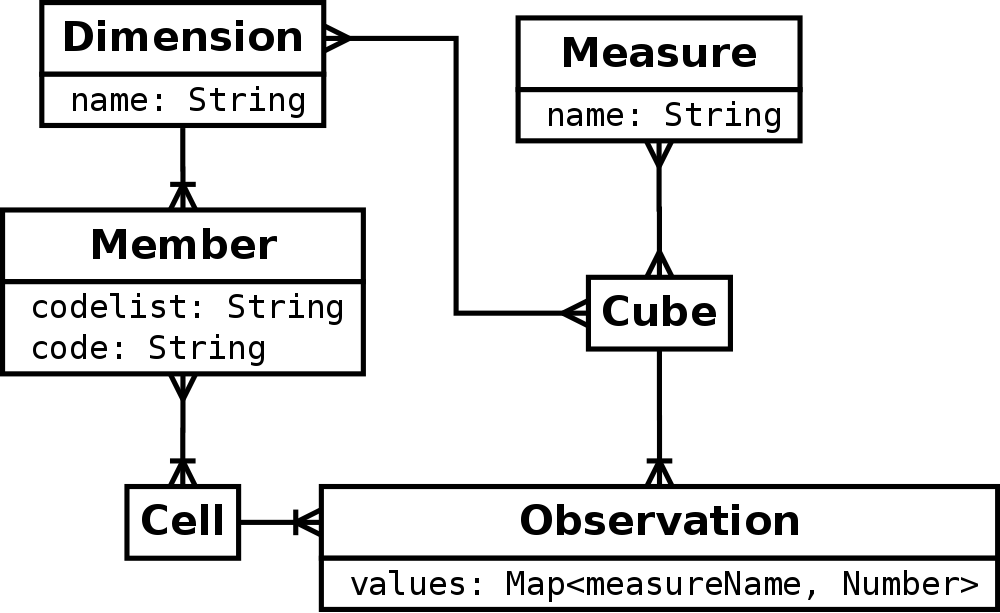
\includegraphics[width=4in]{figs/lds.png}
  \caption [UDC Logical Data Structure]{The Logical Data Structure expressing the representation of Cube Data Sets within the UDC data structure, using the visual data modeling language described in \cite{carlis2000mastering}.}
  \label{fig_lds}
\end{figure}

The following functions transform Data Sets into in-memory representations and help integrate multiple Cube Data Sets together.

\begin{itemize}
\item $createCube(dataset) \rightarrow cube$
\item $createThesaurus(datasets) \rightarrow thesaurus$
\end{itemize}

The $createCube$ algorithm creates a Cube (from figure \ref{fig_lds}) from a Cube Data Set. This procedure must iterate through each Dimension Column and Measure Column of the Data Set to compute the Dimensions and Measures associated with the Cube. Once the metadata has been processed, each row in the relation of the Data Set is transformed into a single Observation. In computing Observations, the requisite Members and Cells are also defined within the in-memory data structure.

The $createThesaurus$ function generates an index that can be used to implement the $canonicalizeMember$ function necessary for merging Cubes. The set of Data Sets input to the $createThesaurus$ function should each be a Concordance Data Set. This means they each have only Dimension Columns that refer to Members of the same Dimension using different Codelists. The relations of Concordance Data Sets serve only to define equivalences between Codes from different Codelists that refer to the same Member. These relations are transformed into an index that maps each $(code, codelist)$ pair to a set of other $(code, codelist)$ pairs that refer to the same Member. The index of equivalence classes can be used in conjunction with a canonical Codelist for each Dimension to implement the $canonicalizeMember$ function. A canonical Codelist can be chosen by sorting all Codelists used in a given Dimension alphabetically and choosing the first one.

\section{Querying Data Sets}
Cubes can be queried by interactive visualizations. Interactive data visualizations need to make a number of different queries for generating user interface components, labels, axes, scales, and visual marks. We assume that a visualization has access to a single Cube containing the integrated data. Starting from the Cube object the following functions provide all queries necessary for general purpose interactive visualizations to operate. This syntax represents functions in terms of their name (before parentheses), what they accept as input (in parentheses), and what they yield as output (after the arrow). Types are denoted as lower case counterparts to UDC concepts, because they represent concrete instances of those concepts.

\begin{itemize}
\item $listDimensions(cube) \rightarrow [dimension]$
\item $listMeasures(cube) \rightarrow [measure]$
\item $listObservations(cube) \rightarrow [observation]$
\item $getValue(observation, measure) \rightarrow \mathbb{R}$
\item $getCell(observation) \rightarrow cell$
\item $member(cell, dimension) \rightarrow member$
\item $slice(cube, cell) \rightarrow cube$
\end{itemize}

The $listDimensions$, $listMeasures$ and $listObservations$ functions list which Dimensions, Measures, and Observations, respectively, are associated with the given Cube. The $getValue$ procedure extracts the numeric value for a given Measure from a given Observation, by evaluating its $values$ property (which maps Measures to numeric values). The $getCell$ procedure reads from the data structure which Cell is associated with the given Observation. The $member$ procedure extracts from the data structure which Member is contained within the given Cell for the given Dimension. The $slice$ procedure implements the traditional OLAP slice operation defined in \cite{datta1999cube}. 

\section{Integrating Data Sets}

The following procedures relate to integrating Cubes:
\begin{itemize}
\item $canonicalizeMember(thesaurus, member) \rightarrow member$
\item $canonicalizeCube(thesaurus, cube) \rightarrow cube$
\item $mergeCubes(cube, cube) \rightarrow cube$
\item $integrate(datasets) \rightarrow cube$ 
\end{itemize}

The $canonicalizeCube$ function transforms a Cube such that all of its Observations use canonicalized Members. When two Data Sets use different Codes to refer to the same Members, the Cubes generated directly from the Data Sets define their Observation domains (Cells) in terms of different Members. A Thesaurus can be used to implement the $canonicalizeMember$ procedure, which resolves equivalent Members referred to using Codes from different Codelists. The $canonicalizeCube$ function invokes $canonicalizeMember$ as a subroutine to normalize the Observations of the Cube. After running $canonicalizeCube$ on two Cubes that use different Codelists, both resulting Cubes use the same Codes to refer to the same Members. This step enables the two Cubes to be merged using $mergeCubes$.

The $mergeCubes$ procedure joins the Observations from two Cubes by matching on their Cells. Each Cell is identified by a unique set of Members. Cells from both Cubes match because the $canonicalizeCube$ procedure was invoked previously on each input cube. In implementing $mergeCubes$, one could employ an inner join strategy, which would yield a Cube with no missing data but may not include all of the original data, or an outer join strategy, which would yield a Cube with missing data (Observations with missing values for some Measures) but would include all of the original data.

Figure \ref{fig:integration} shows the \emph{integrate} algorithm for integrating many Data Sets. This algorithm first transforms all Cube Data Sets in the input $datasets$ array into Cubes using $createCube$, and constructs a Thesaurus from all Concordance Data Sets in the input $datasets$ array using $createThesaurus$. A map-reduce pattern is then applied to integrate all Cubes. The map portion of the algorithm applies the $canonicalizeCube$ function to all Cubes, using the already created Thesaurus to canonicalize Members used in each Cube. The reduce portion of the algorithm applies the $mergeCubes$ function to merge all canonicalized Cubes recursively. The result from the entire algorithm is a Cube that contains data from all of the input Cubes combined and integrated properly. The resulting Cube is suitable for input into interactive visualizations.

\begin{figure}
  \centering
  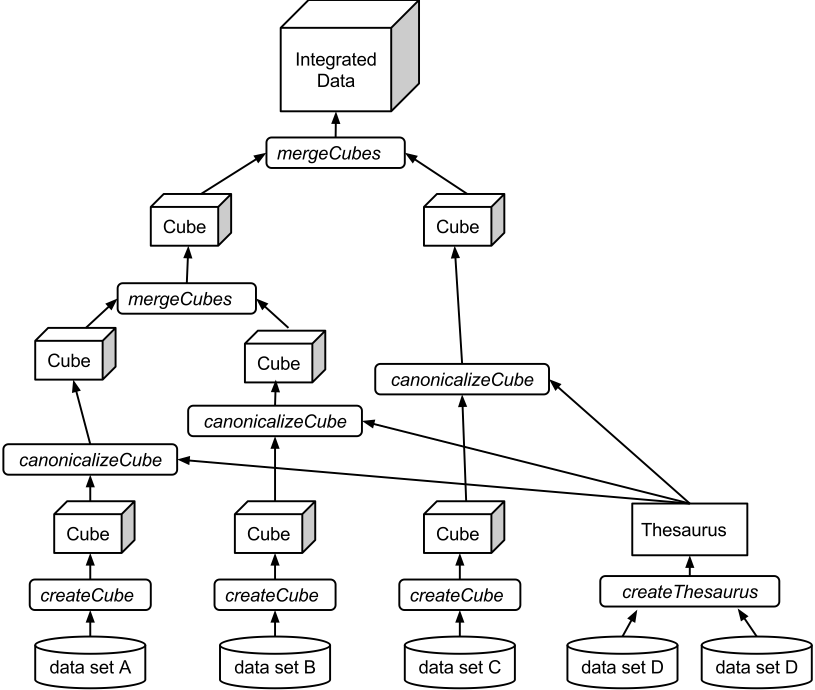
\includegraphics[width=\figureWidth]{figs/integration.png}
  \caption [UDC Data Integration Algorithm]{The flow of the $integrate$ algorithm for integrating data.}
  \label{fig:integration}
\end{figure}

\section{Limitations of Data Cube Representation}
Many, but not all, data sets can be modeled as data cubes. Since data cubes are only capable of representing data that has been aggregated along categorical dimensions, there are many classes of data that do not fit within the conceptual framework of data cubes. For example, a database containing the details of transactions in a supermarket would not be appropriate to model as a data cube. Each entry of a customer purchase may contain a listing of items purchased, how it was paid for, and the date and time the purchase was made. This kind of data fits well into the relational model, but is not appropriate to model as a data cube. Data cubes represent only aggregated summaries, not individual events. In the case of grocery store database containing the transactions for many grocery stores in different regions, while the individual transaction entries cannot be modeled as a data cube directly, a data cube can be constructed from the transactional data by aggregating measures such as ``amount paid'' and ``number of items purchased'' along dimensions such as ``time'', ``region'' and ``product category''. This is a typical data warehouse scenario, where a business aggregates transactional data into a data cube in order to analyze company activities in a summary view.

The key characteristics that allow a given data set to be modeled as a data cube are as follows:

\begin{itemize}
\item The data set contains numeric fields that represent aggregated summaries using sum, average, or some other aggregation operator (measures).
\item The measures of the data set are aggregated along one or more sets of discrete categories or entities (dimensions).
\end{itemize}

Dimensions can be either unordered, ordered, or hierarchical. Dimensions include Space, defining hierarchies of geospatial regions, Time, defining intervals in time, or of any arbitrary collection of categories. Examples of dimensions other than Time and Space include Gender, Ethnicity, and Industry. The Space dimension can be decomposed using several alternative strategies. The most common spatial decomposition found in data is along geopolitical boundaries. Another way to decompose spatial regions is according to a quadrilateralized spherical cube, also called a quad sphere \cite{tobler1986quadtree}. The quad sphere approach provides uniformly distributed regions at multiple levels of detail, which makes it appropriate for presenting aggregated summaries of more detailed data such as billions of points on Earth or satellite imagery data \cite{white1992quadrilateralized}. Yet another alternative geospatial partitioning strategy is by global river basins. Partitioning data by river basins makes sense for climate and weather related data \cite{worldbank2014climate}.

Data sets that have the following qualities may not be modeled directly as data cubes.
\begin{itemize}
\item The data set represents a graph. Graph data such as social network connections or links between Web pages is not supported by the data cube model.
\item The data set contains relational data with a one-to-many relation. For example, a database of transactions in a grocery store where one transaction has many items. Items containing lists of other items cannot be represented using the data cube model. However, one may consider transforming data sets like this such that the nested lists are summarized by some measures (such as total cost or number of items) so the data cube model can be applied.
\item The data set contains entries for individual discrete events or transactions. Data sets with this quality cannot be modeled directly as data cubes, however it may be possible to compute data cubes by aggregating them using OLAP techniques from data warehousing.
\end{itemize}

Although data sets with the above qualities may not be modeled directly as data cubes, it may be possible to compute data cubes that summarize data sets like these. For example, the BrightKite data set which was originally structured as a graph \cite{cho2011friendship} can be aggregated using the data cube approach then visually analyzed \cite{liu2014effects, liu2013immens}. Any graph data set in which nodes contain metadata such as location and time can be aggregated along Space, Time and other dimensions to form a data cube.

\section{Proof of Concept}

The United Nations (UN) Population Prospects Data Set provides population data for each country of the World over time. A small sample of this data set is shown in table \ref{table_unPop}. This data set was downloaded as an Excel spreadsheet (shown in figure \ref{fig:unPopExcel}), exported as a Comma Separated Value (CSV) file, then transformed to be in the format expected by a data cube dataset (one row for each Observation). This data set uses the UN M.49 country codes to refer to countries. Figure \ref{fig:unTimeline} shows a slice of this data set showing population values over time for the entire world. This visualization gives a broad overview of the data. By drilling down, lines in the line chart can be made to represent individual countries.

\begin{figure}
  \centering
  \includegraphics[width=\figureWidth]{figs/UN_World_Population_Spreadsheet.png}
  \caption [United Nations Population Prospects Data Set]{The United Nations Population Prospects data set \cite{unPopData}, made available in Excel format. This is an example data set that can be imported into our data structure and integrated with other data sets.}
  \label{fig:unPopExcel}
\end{figure}

\begin{figure}
  \centering
  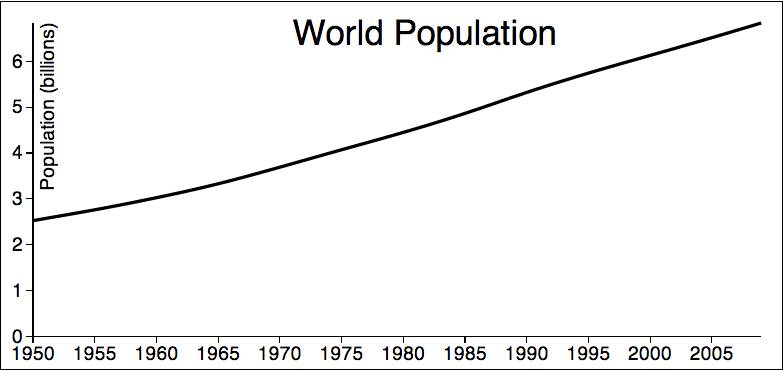
\includegraphics[width=\figureWidth]{figs/unTimeline.png}
  \caption [World Population Timeline]{A timeline visualization of the United Nations Population Estimates data set. This shows the population of the entire world from 1950 to 2010.}
  \label{fig:unTimeline}
\end{figure}

The World Bank publishes publicly available data about a number of topics. One dataset from the World Bank contains the Gross Domestic Product (GDP) of each country over many years, shown in figure \ref{fig:worldBankGDP}. A small sample of this data set is shown in table \ref{table_gdp}. This data set uses the ISO3 standard Codelist for countries.

\begin{figure}
  \centering
  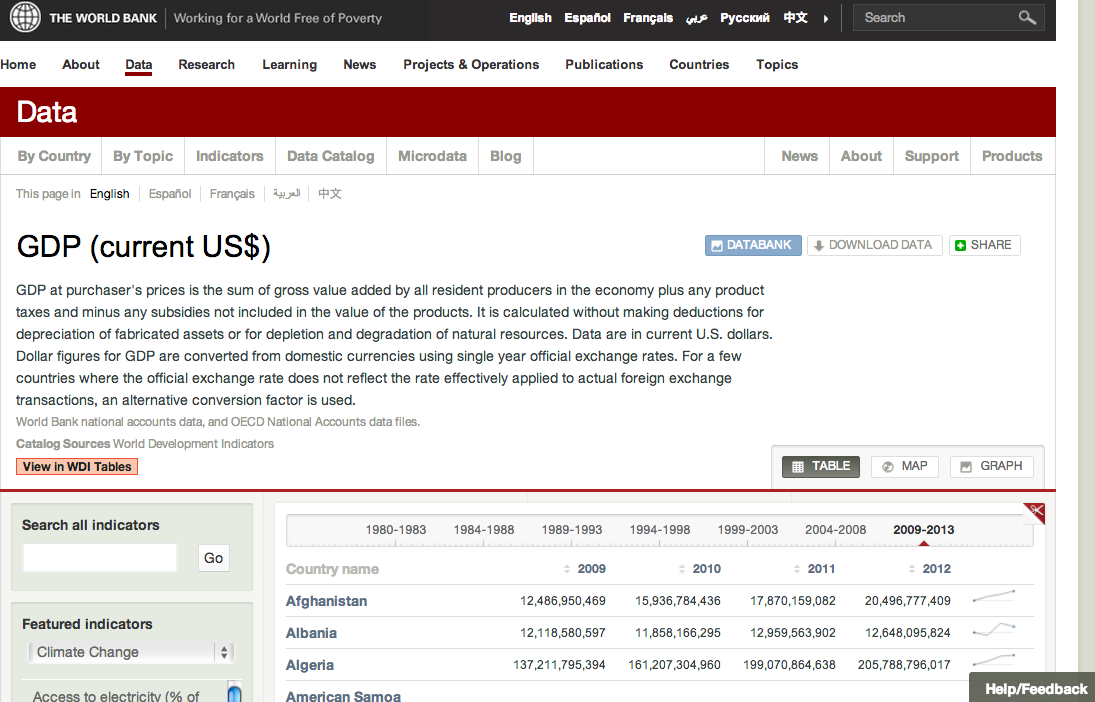
\includegraphics[width=\figureWidth]{figs/worldBankGDP.png}
  \caption[World Bank GDP Data Set]{The World Bank GDP Data Set.}
  \label{fig:worldBankGDP}
\end{figure}

We applied the UDC approach to modeling and integrating the UN Population Prospects data set and the World Bank GDP data set. The resulting integrated Cube was visualized as a scatter plot, shown in figure \ref{fig:scatter}. In this visualization, Population is mapped to the X axis, GDP is mapped to the Y axis, and each dot represents a country. Both axes are log normalized in order to spread the data. This plot shows that there is a correlation between Population and GDP, and that both measures follow roughly a Power Law distribution. This demonstrates a proof of concept implementation of the UDC data structure and algorithms for integrating and visualizing public data.

Consider the steps required to produce the scatter plot visualization of the integrated Population and GDP Cube shown in figure \ref{fig:scatter}. First, the dimensions of the integrated Cube, namely Time (Years) and Space (Countries), can be computed using the $listDimensions$ function. Since we want each dot to represent a country, the Cube must then be sliced using the $slice$ function such that it contains only data for a single year. Next, the X and Y scales must be defined. The $listMeasures$ procedure can be used to generate a list from which users can choose which measures to assign to the X and Y axes. Once X and Y measures are chosen, the $listObservations$ procedure can generate the list of Observations to transform into visual marks (one for each Country). To compute the domains for the X and Y scales, the Observations can be queried for their X and Y measure values using the $getValue$ procedure. The minimum and maximum values returned for the X and Y measures can define the domains for the X and Y scales. Once the scales have been defined, the Observations can be iterated over once more to generate the complete visualization. This is one example of how the given query algorithms for Cube Data Sets can be used for visualization. 

\begin{figure}
  \centering
  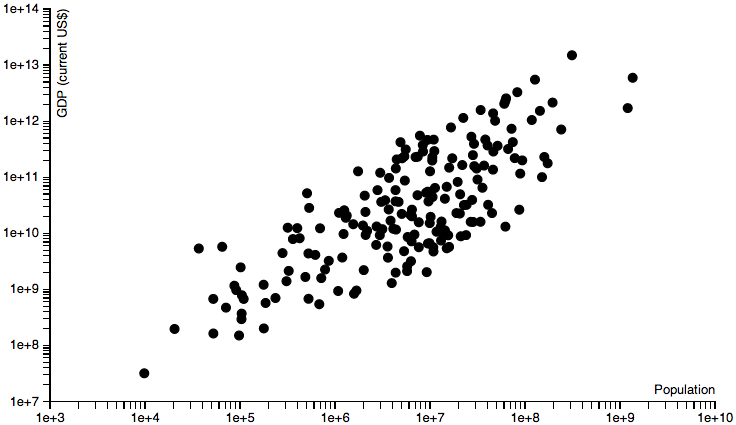
\includegraphics[width=\figureWidth]{figs/scatter.png}
  \caption[Scatter Plot of Integrated Data]{A scatter plot visualizing two data sets integrated together. The X axis shows Population, drawn from a United Nations data set, and the Y axis shows GDP, drawn from a World Bank data set. Each dot represents a country.}
  \label{fig:scatter}
\end{figure}

The $slice$ procedure can be utilized for developing visualizations with multiple linked views. This is when one visualization shows an overview, and interactions in that visualization can define how the input data for another visualization is sliced before it is visualized. We have implemented a prototype of this concept which uses a linked Choropleth Map and Line Chart, shown in figure \ref{fig:choropleth}. Zooming in the Choropleth Map defines the set of countries represented as lines in the Line Chart. Selecting a year in the Line Chart causes the Choropleth Map to show data for that year only.

\begin{figure}
  \centering
  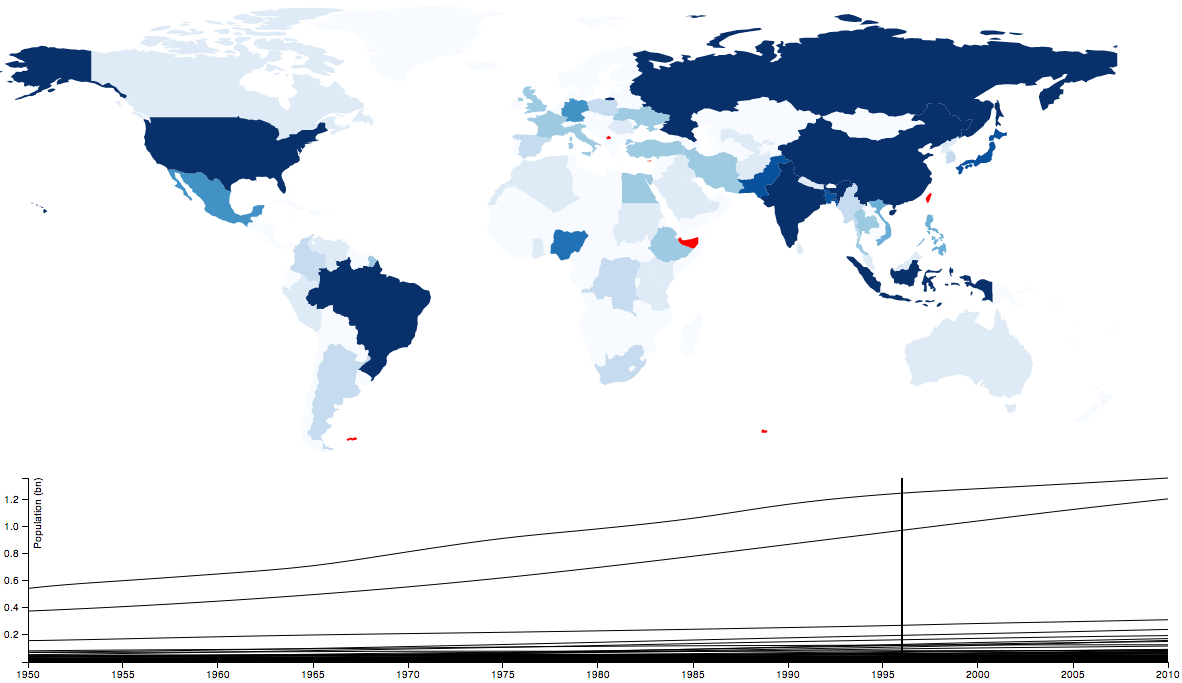
\includegraphics[width=\figureWidth]{figs/choropleth.png}
  \caption [Linked Line Chart and Choropleth Map]{A linked line chart and Choropleth map showing population data from the United Nations. Zooming in the map filters the line chart. Selecting a year in the line chart causes the map to show data from that year. This demonstrates how the $slice$ procedure can be utilized for generating interactive visualizations with linked views. Red indicates missing data.}
  \label{fig:choropleth}
\end{figure}

\section{Crowdsourcing Data Experiment}
Rather than manually curating data, a crowdsourcing approach can be taken to data collection for the UDC. We have performed an initial experiment to test the feasibility of this approach. Amazon Mechanical Turk supports assignment of tasks, called ``Human Intelligence Tasks'' or HITs, to workers who get paid small amounts (on the order of cents) to execute the tasks. To populate the UDC using Mechanical Turk, HITs can be devised that ask workers to find an answer to a simple question like ``What was the population of India in 1950?''. This question is an instance of a more general form ``What was the \verb1${measure}1 of \verb1${place}1 in \verb1${time}1''. By enumerating possible values for \verb1${measure}1, \verb1${place}1, and \verb1${time}1, responses to such HITs can populate large regions of the UDC.

To test the crowdsourcing data collection approach, an experiment was performed using Amazon Mechanical Turk. In this experiment, \verb1${measure}1 = population, \verb1${place}1 = \{India, China, United States\}, and \verb1${time}1 = \{1950, 2010\}. The results contained between 7 and 10 responses from multiple workers for each combination of place and time. By taking the mode (most frequently occurring value) of the worker submissions for each combination of place and time, the following table was generated:

\begin{figure}[h!]
  \centering
  \begin{tabular}{ | l | l | l | l | }
  \hline
  Place & Time & Population & Source URL \\ \hline
  India & 1950 & 369880000 & \tiny \verb1www.geohive.com/earth/population3.aspx1 \\ \hline
  China & 1950 & 563000000 & \tiny \verb1geography.about.com/od/populationgeography/a/chinapopulation.htm1 \\ \hline
  USA & 1950 & 150697361 & \tiny \verb2en.wikipedia.org/wiki/1950_United_States_Census2 \\ \hline
  India & 2010 & 1150000000 & \tiny \verb1www.indiaonlinepages.com/population/india-population.html1\\ \hline
  China & 2010 & 1339724852 & \tiny \verb1en.wikipedia.org/wiki/Demographics_of_China1\\ \hline
  USA & 2010 & 308745538 & \tiny \verb1en.wikipedia.org/wiki/United_States_Census1\\ \hline
  \end{tabular}
  \caption[Mechanical Turk Results]
   {Initial results from an experiment in crowdsourcing public data using Amazon Mechanical Turk.}
  \label{fig:crowdData}
\end{figure}

In the table shown in figure \ref{fig:crowdData}, each row represents an observation within the data cube. The values in the Place column refer to members of the Space dimension. The values in the Time column refer to members of the Time dimension. The values in the Population column assign numeric values to cells (combinations of Space and Time members) for the Population measure. This initial result demonstrates the feasibility of crowdsourced data collection for the UDC.

\section{Summary}
This chapter introduced novel data structures and algorithms for integration of multiple data sets, and for querying the merged data structure for use in interactive visualizations. We call this collection of data structures and algorithms the Universal Data Cube (UDC). This approach functions by using concordances to canonicalize identifiers used across data sets, then merging data cubes in a map-reduce fashion. The resulting integrated structure can be queried for generation of interactive visualizations. Future work will focus on developing reusable interactive visualizations that can use the UDC data structure as input, and on a framework for easily assembling linked views based on the UDC data structure.



\chapter{Conclusion}
Data today is growing in both size and variety. By modeling the data within a data cube based framework, it is possible to tame the vast collection of various representations of complex data into a predictable structure. This simplified data model imposes structural restrictions on the data, and in doing so makes the data more amenable to interactive visual analysis.

\section{Contributions}

The contributions of this dissertation are novel data structures and algorithms covering a broad range of the data visualization pipeline. The Universal Data Cube data model is an attempt at providing a data model that both captures the essence of many data sets and exposes a simple and predictable data structure upon which interactive visualization systems can be built. The Reactive Visualization approach is the first to synthesize the Model View Controller paradigm with functional reactive programming to construct reusable interactive visualization components. Dynamic visualization configuration allows reusable visualizations to be instantiated within the context of many data sets and allows users to collaborate in real time over interactive visualizations. Taken together, these contributions represent a new approach to the process of integrating and visualizing data.

Reactive models provide the foundation for reactive visualizations. This approach allows the construction of reusable reactive flows that encapsulate elements of interactive visualizations. Using reactive flows, much of the data visualization pipeline can be implemented. Reactive flows enable representation of update flows from data and configuration through to visualization scales, axes and visual marks. In theory, any imaginable visualization technique can be implemented as a reactive visualization component. The prototypes presented in this dissertation serve as a starting point for a growing catalog of Open Source visualization modules.

Interactions such as brushing, picking and zooming can also be encapsulated using reactive models. The interactions in one visualization can be used to drive interactive changes in other visualizations. In this way visualizations with multiple linked views can be constructed. Interaction schemes for linked views include dynamic filtering, slicing, linked selection and linked probing. For example, zooming in a map can filter the regions used to filter the input to a line chart of population. This technique of using interaction for dynamic slicing can be used to build data cube exploration tools that replace small multiples with interactive linked views.

An application state model based on reactive models provides the foundation for a collaborative visual data exploration platform. Application state configuration based on JSON enables configuration of visualizations with multiple linked views. A unique runtime engine is introduced for configurable applications that dynamically loads required modules. Using this framework it is possible to author and evolve instantiations of reusable visualization components with linked views. The application state model also affords construction and navigation of history graphs supporting undo, redo, and view sharing.

The Universal Data Cube framework proposes a framework for representing data based on the data cube model. This framework is ``universal'' in that it is capable of representing aggregated summaries of any measurable quantity over limitless time and space. The Time and Space dimensions provide conceptual delineations between regions of hierarchical time and space. Measures provides windows into phenomena occurring within certain regions of time and space. In theory, all measurable quantities that summarize events and phenomena can be represented using this framework. The limited Open Source proof of concept implementation of the UDC framework is proposed as the seed for a large ongoing project aimed at curating and exposing public data.

By combining the data curated within the UDC and the proposed visualization and collaboration frameworks, the aim is to provide a complete platform for data visualization. The hope is that this platform will enable Web users and content creators to easily investigate any data of interest using interactive data visualization. Application areas for this technology include commercial data analysis, business intelligence, education, journalism and public policy.
% Notes from 10/9 Haim MTG
% Collaboration real contributions? Talk more about collaboration.
% This is marketing "I've done something that is new"
% Brag about it.

% What one could have done but I didn't do.

\section{Future Work}
The realization of this work so far is far from the complete vision. The vision is to establish a Wikipedia-like platform for collaborative data visualization. The technologies presented in this dissertation provide the foundation for such a system, but more work needs to be done to glue the pieces together into a complete and coherent suite of tools.

The reactive model solution introduced has the potential to be formalized as a time tick based execution system. This kind of formalization would allow a rigorous asymptotic analysis of reactive models based on their data flow graph structure. For example, one could quantify the influence of various graph characteristics such as total number of nodes and breadth first search tree distance from a node that is the source of a change. 

The Universal Data Cube data model has the potential to be implemented within a database. This would involve the construction of a database schema that persists the UDC model and allows users to query the data present. The overall effect of maintaining a UDC database is that common dimensions and measures will become clear. Given a collection of 100 data sets, a UDC database could keep track of the total list of all dimensions and all measures. For each dimension, the database could tell you how many data sets use it, and what the most common key codes are. The database could also provide information about measures such as how many measures there are, how many data sets cover each measure, and what dimensions and members are covered by each measure. These kinds of queries could be coupled with visualization interfaces to present a rich overview of a large collection of data and support unprecedented visual data exploration capabilities.

The envisioned collaboration framework would be a database driven Web application enabling users to import their own data, add their own reusable visualization components, and collaboratively author interactive visualizations. User interfaces supporting these operations must also be developed. For importing data sets, a simple solution similar to the ManyEyes data import user interface would suffice \cite{viegas2007manyeyes}. For adding reusable visualization components, an in-browser code editing tool with versioning would be required (similar to JSBin). For collaboratively authoring interactive visualizations, the dynamic configuration structure can be linked with an operational transformation system such as ShareJS or Firebase. States of interest must be persisted to a database for later viewing or further editing. Existing collaboration platforms that already track data sets such as OpenChorus \cite{openChorus} could be extended to include interactive visualizations. The visualization state created by users can be simply persisted as a string in the application database.

The UDC visualization technology can be extended to accommodate real time updating data. This could be accomplished by polling for data updates or using a server push technology such as WebSockets. For updating data, the data values of the most recent time slice of the data cube may change. For granular time slices such as hours or days, new Time dimension members are created as time passes, so new slices of the data cube could be sent from the server to clients as they become available.

Mobile technology could be one of the largest targets for interactive visualization technology. For example, many readers of popular news feeds such as the New York Times consume their content using mobile devices such as smart phones, phablets and tablets. The same is true for E-Books and blogs. With this in mind, considerations must be made regarding how to tailor the proposed interactive visualizations to mobile devices with touch screen interfaces and variable resolution.

Only a few reusable visualization components have been implemented and a few data sets imported into the framework so far. The following sections discuss development of more reusable visualization components, more interaction techniques, and importing of more data sets into the UDC framework.

\section{Visualizations and Interactions}
The complete set of visualization techniques suitable for adaptation as reusable components is vast. Bertin enumerates the numerous possibilities for visually encoding data \cite{bertin1983semiology}. This is why an expandable user-driven platform is more suitable than a fixed set of visualizations. As a first step toward the goal of an open platform with the potential to accommodate any imaginable visualization technique, an initial set of visualization techniques are presented here in table \ref{table_data_cube_visualizations}.

These visualizations can be augmented by interaction techniques such as brushing, picking, hovering, pan and zoom. Each of these interactions results in a user defined subset of the data visualized. The output from the interaction in any visualization can be used to slice or filter the input of another. Brushing involves the interactive visual definition of a rectangular region that defines intervals in data space. The intervals defined by a brush region can be used to filter the original data, allowing users to interactively define subsets of the data. Picking involves tapping or clicking on a single visual mark. Hovering (also called probing) selects the single visual mark closest to the mouse. Hovering can use a Voronoi overlay to improve performance. Panning and zooming can be used on a geographic map to define a subset of regions. Conceivably, pan and zoom could also be implemented in other visualizations such as scatter plot.
\newcommand{\thumbnailWidth}{1.2in}
\newcommand{\descWidth}{2.9in}
\newcommand{\descPadding}{\vspace{.3\baselineskip}}

\begin{table*}
  \caption{Reusable Data Cube Visualizations.}
  \centering
  \label{table_data_cube_visualizations}
  \begin{tabular}{ | c | c | c |}
    \hline
    \textbf{Name}
      & \textbf{Thumbnail}
      & \textbf{Description} \\ \hline

    Bar Chart

      & \parbox[c]{\thumbnailWidth}{\centering 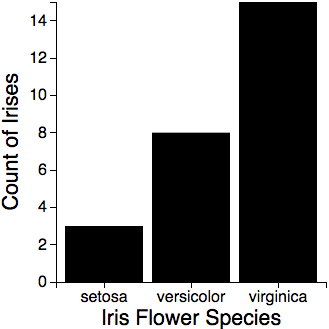
\includegraphics[width=\thumbnailWidth]{figs/visThumbnails/barchart.png}}
      & \parbox[c]{\descWidth}{\descPadding
        1 Dimension (bar) \\
        1 Measure (bar height) \\
        Optionally: \\
        Picking interaction (click on bar)
      \descPadding} \\ \hline

    Pie Chart

      & \parbox[c]{\thumbnailWidth}{\centering 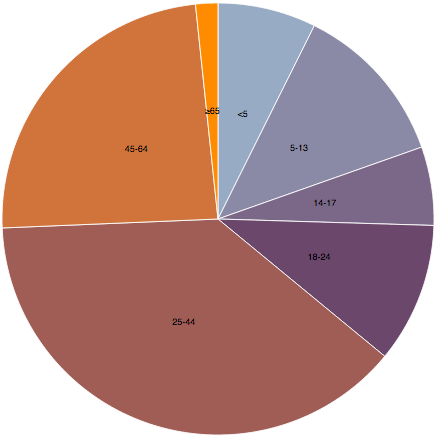
\includegraphics[width=\thumbnailWidth]{figs/visThumbnails/pie.png}}
      & \parbox[c]{\descWidth}{\descPadding
        1 Dimension (slice) \\
        1 Measure (slice size) \\
        Optionally: \\
        Picking interaction (click on slice)
      \descPadding} \\ \hline


    Scatter Plot

      & \parbox[c]{\thumbnailWidth}{\centering 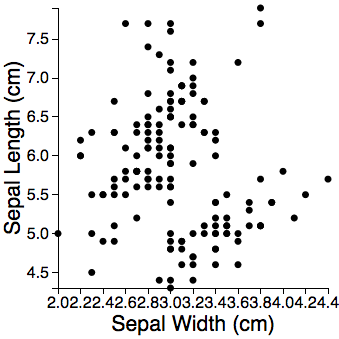
\includegraphics[width=\thumbnailWidth]{figs/visThumbnails/scatterplot.png}}
      & \parbox[c]{\descWidth}{\descPadding
        1 Dimension (mark) \\
        2 Measures (X, Y position) \\
        Optionally: \\
        +1 Dimension (symbol) \\
        +1 Measure (size) \\
        +1 Measure (color) \\
        Brushing interaction (2D)
      \descPadding} \\ \hline

    Parallel Coordinates

      & \parbox[c]{\thumbnailWidth}{\centering 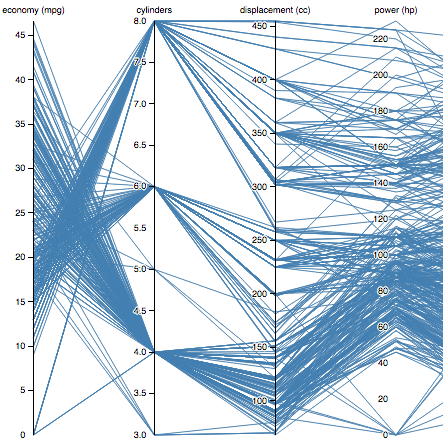
\includegraphics[width=\thumbnailWidth]{figs/visThumbnails/parallelCoords.png}}
      & \parbox[c]{\descWidth}{\descPadding
        1 Dimension (polyline) \\
        N Measures (one for each parallel axis) \\
        Optionally: \\
        Brushing interaction for each axis
      \descPadding} \\ \hline

    Choropleth Map

      & \parbox[c]{\thumbnailWidth}{\centering 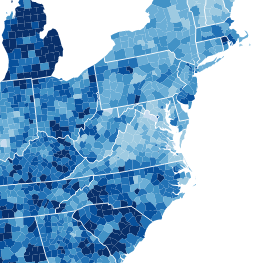
\includegraphics[width=\thumbnailWidth]{figs/visThumbnails/choropleth.png}}
      & \parbox[c]{\descWidth}{\descPadding
        1 Dimension, Space (geographic region) \\
        1 Measure (color) \\
        Optionally: \\
        Small multiples visualization overlay \\
        Picking interaction (click on region) \\
        Pan \& Zoom interaction
      \descPadding} \\ \hline
  \end{tabular}
\end{table*}

\begin{table*}
  \caption{Reusable Data Cube Visualizations (continued).}
  \centering
  \begin{tabular}{ | c | c | c |}
    \hline
    \textbf{Name}
      & \textbf{Thumbnail}
      & \textbf{Description} \\ \hline

    Sunburst

      & \parbox[c]{\thumbnailWidth}{\centering 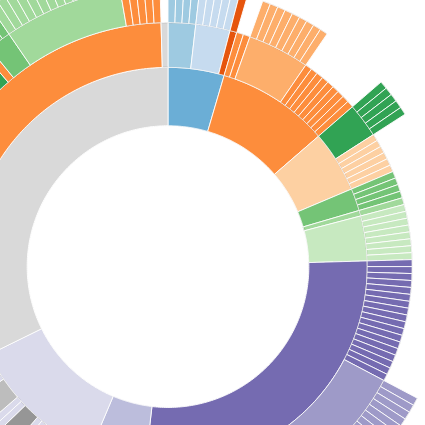
\includegraphics[width=\thumbnailWidth]{figs/visThumbnails/sunburst.png}}
      & \parbox[c]{\descWidth}{\descPadding
        1 Dimension, Hierarchical (slice) \\
        1 Measure (slice size) \\
        Optionally: \\
        Picking interaction (click on slice)
      \descPadding} \\ \hline

    Icicle

      & \parbox[c]{\thumbnailWidth}{\centering 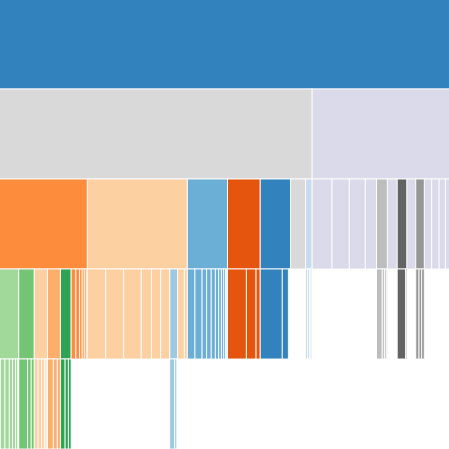
\includegraphics[width=\thumbnailWidth]{figs/visThumbnails/icicle.png}}
      & \parbox[c]{\descWidth}{\descPadding
        1 Dimension, Hierarchical (rectangles) \\
        1 Measure (rectangle length) \\
        Optionally: \\
        Picking interaction (click on rectangle)
      \descPadding} \\ \hline

    TreeMap

      & \parbox[c]{\thumbnailWidth}{\centering 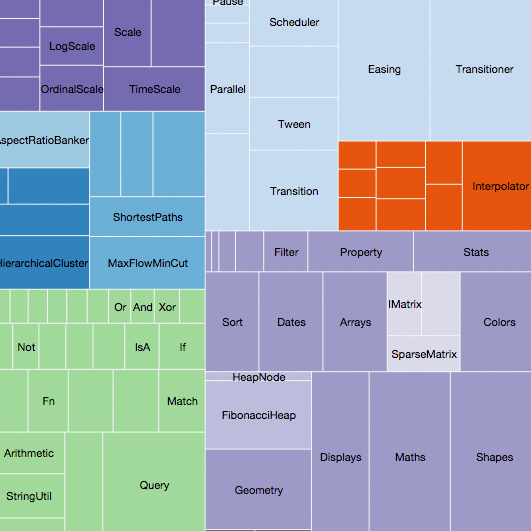
\includegraphics[width=\thumbnailWidth]{figs/visThumbnails/treemap.png}}
      & \parbox[c]{\descWidth}{\descPadding
        1 Dimension, Hierarchical (rectangles) \\
        1 Measure (rectangle area) \\
        Optionally: \\
        Picking interaction (click on rectangle)
      \descPadding} \\ \hline

    Streamgraph

      & \parbox[c]{\thumbnailWidth}{\centering 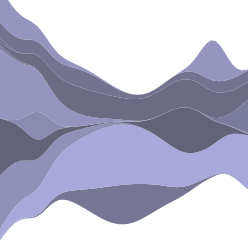
\includegraphics[width=\thumbnailWidth]{figs/visThumbnails/streamgraph.png}}
      & \parbox[c]{\descWidth}{\descPadding
        2 Dimensions, (Time, streams) \\
        1 Measure (stream thickness) \\
        Optionally: \\
        Picking interaction (click on stream), or
        Picking interaction (click on time), or
        Brushing interaction (across Time)
      \descPadding} \\ \hline

%streamgraph
%sunburst

%brushing
%donut
%embeddedGeoVisualizations
%picking
%pie
%stackedArea
%stackedBars
%table
%temporalBrushing
%treemap
  \end{tabular}
\end{table*}

\section{Data Sources}

There are numerous rich data sources on the Web that are suitable for import into the Universal Data Cube framework for visualization. So far only a few data sets have been actually imported, however many have been evaluated and identified as candidates. Some data sources provide archives of historical data, while others are vastly large and expose the data via a Web API. Crowdsourcing platforms also present immense potential for finding data sources and curating data.

The Pew Global Religious Landscape data set provides data about religious composition by country. This data set covers dimensions of Time (only the 2010 slice is provided), Space (countries), and Religion. The measure can be modeled as Population, as the addition of the Religion dimension effectively is a filter through which to view the population of a place. This data set can be enhanced by integration with a data set providing population data for each country of the World in 2010.

For each country, it is possible to visualize the data cube slice for that country as a bar chart in which each bar represents a religion. Therefore a visualization with linked views can be assembled in which picking interaction in a choropleth map can drive the country used as input for the bar chart. Clicking on each country would show its religious profile as a bar chart. This linked visualization would use the map to visualize and navigate the Space dimension, and the bar chart to visualize the Population measure by the Religion dimension. Together, the map and bar chart could visualize a data cube with 2 Dimensions (Space, Religion) and 1 Measure (Population). The original data cube included the Time dimension as well, which effectively gets eliminated by taking only the 2010 slice as input. If historical data were available for each year, a line chart could be paired with the linked visualization to visualize and navigate the Time dimension.

The Religious Landscape data set can also be visualized as bar charts (or pie charts, or donut charts) overlaid on a geographic map. The bar charts can be squares with area representing population. Each bar within the square represents a religion. By pairing size of the bar chart with population, area corresponds to quantity of people accurately. In other words, each pixel on the screen inside a bar represents a fixed number of people. Visually, this makes sense because the human visual system naturally experiences and assesses sizes of things based on their area. \cite{tufte1983visual} Pie charts could also be overlaid on a geographic map to express the same information.

Whether pie charts or bar charts, the embedded visualizations are at risk of occluding each other when plotted directly centered at the centroid of their corresponding regions. This can be overcome by using a force directed layout that repels embedded visualizations away from one another such that each is fully shown and not occluded by others. A similar technique has been used previously in cartography to produce cartograms based on circles (Dorling Cartogram) and squares (Demers Cartogram) \cite{tobler2004thirty}.

Note that the geographic visualization overlay presents the same information as the above described linked map and bar chart interactive visualization. Rather than clicking on a country, the user can now just look at the center of any given country on the map to assess its religious breakdown. In this way, the geographically overlaid visualizations communicate more information at a time than the linked views. 

The geographic bar chart visualization could also be augmented by a line chart if historical data is also available. The line chart could visualize the Time Dimension as a streamgraph chart showing global religious breakdown over time. Picking interaction for years in the streamgraph can define the Time slice used as input to the other visualizations. This is one example of the general case that adding another visualization with picking interaction can effectively add another dimension to the data space users are capable of navigating with the visualization interface.


%Data APIs e.g. World Bank, CDC, WHO
%
%MDG
%
%BLS
%
%Eurostat
%
%Census
%
%ACS
%
% http://www.worldmapper.org/data.html



DBPedia is a knowledge graph representation of Wikipedia. DBPedia data is represented using RDF (Resource Description Framework), the World Wide Web Consortium standard knowledge graph representation for the Semantic Web \cite{klyne2006resource}. In DBPedia, each Wikipedia Page about an entity is classified according to the DBPedia Ontology \cite{bizer2009dbpedia}. Resources in DBPedia can be aggregated along the DBPedia Ontology to produce a data cube that can be visualized. For example, one could visualize the count of resources for each ontology class using a Sunburst or Icicle visualization. Since resources have (lat, long) coordinates and associated dates, they can also be aggregated along Space and Time.

OpenStreetMap (OSM) is a community maintained crowdsourced geographic data repository \cite{haklay2008openstreetmap}. The OSM database contains entities of numerous types including roads, points of interest, educational institutions, churches, buildings, military bases, shops, and public transit stations \cite{osmMapFeatures}. Any of these types can be counted across geographic space and used as indicators. For example, the number of buildings can be used to approximate population at a high resolution. Map features can also be aggregated by type and visualized to show the breakdown of the database.

The 2014 global Ebola outbreak is being monitored closely. Structured data about the outbreak is available and updating every day. This data provides measures ``number of Ebola deaths'' and ``number of Ebola cases'' for each affected West African nation for each day since the outbreak began. The New York Times published a graphical piece including a small multiples visualization of Ebola \cite{nytEbola}. This is a topic prominent in the news today. A dynamically updating visualization for this data would be indispensable for journalists and decision makers alike.

The Global Terrorism Database provides historical data about terrorist activities such as attacks with their time, place, and number of deaths. With daily news on ISIL (Islamic State of Iraq and the Levant), this live updating data set is a valuable resource for many people including journalists, policy makers, or anyone interested in learning about terrorist related events. This data can be aggregated into a data cube covering dimensions Time (nested structure of years, months, days), Space (geographic region), and providing the measure of number of deaths. This data could be visualized as a linked line chart and choropleth map. Picking in the line chart slices data used as input to the choropleth map. Zooming in the choropleth map dices the data shown in the line chart. This is similar to the linked view visualization of population described in figure \ref{fig:choropleth}.


\begin{figure}
  \centering
  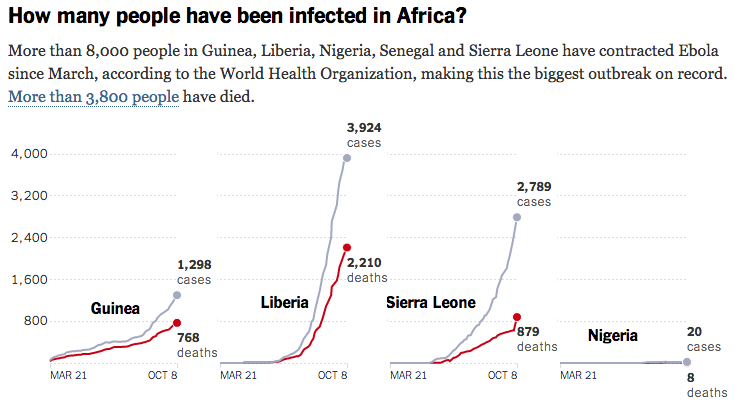
\includegraphics[width=\figureWidth]{figs/nytEbolaLines.png}
  \caption [New York Times Ebola Visualization]{ A small multiples line chart visualization of the 2014 Ebola outbreak in West Africa published by the New York Times \cite{nytEbola}. This visualization shows the number of Ebola cases and deaths by day by region.}
  \label{fig:nytEbolaLines}
\end{figure}

Crowdsourcing may also be a promising approach for collecting and curating data. Each combination of region, time and measure can be formulated as an English question, such as ``What was the GDP of India in 1970?''. Crowdsourcing platforms such as Amazon Mechanical Turk and Crowdflower can potentially be utilized to collect data. Workers may also be asked to enter the URL from which they found the data value. These URLs can be used to glean the structure of what is covered by various data sources, which can in turn be used to suggest URLs to future workers for certain regions of the data cube structure. Using this approach, it may be possible to develop an automated service that collects requested data on demand. Crowdsourcing techniques can also be used to refine the quality of the data collected.

\section{A Grammar of Graphics Approach}
A system based on named visualizations (e.g. "Scatter Plot", "Bar Chart") allows each visualization to have their own implementation, and does work. However, this approach is limited in that it does not take advantage of the deeper structure of visualizations. Leland Wilkinson's "Grammar of Graphics" describes a language for expressing many types of visualizations using a single grammar \cite{wilkinson2005grammar}. Hadley Wickham has implemented this grammar and extended it in the R package \verb1ggplot21 \cite{wickham2010layered, wickham2009ggplot2}. A JSON-based grammar of graphics called VisJSON has also been developed \cite{vizJSON}.

Incorporating a grammar of graphics implementation into the proposed visualization platform would allow configuration of powerful and complex linked visualizations using a minimally complex structure. Each visualization on a page could be described by a grammar of graphics expression, rather than invoking a module that implements a named visualization. This kind of system would be much more elegant. One additional benefit of this organization is that when new features such as interaction techniques are implemented in the grammar of graphics engine, all visualizations immediately have the new interaction available. In a named visualization system, the interaction would need to be implemented once per visualization module.

One path to a grammar of graphics based approach within the existing reactive visualization framework is to create a grammar based solution that can express incrementally more visualizations. In this sense, it is essential to first have developed a named visualization approach, then start on the grammar of graphics approach. For example, a grammar of graphics based solution can be introduced that first can generate a scatter plot, then a bar chart, then a pie chart, then a stacked bar chart. As the implementation grows in completeness, named visualizations can be incrementally replaced with expressions in the grammar.

\section{Final Thoughts}
The hoped for eventual impact of this work is to enable common everyday people to understand their world better through data visualization. By providing a basis on which complex interactive visualization systems can be built and tailored to the data at hand, this work paves the way for future researchers and developers to create visualizations that represent data clearly and can be understood by many. Whether seen on a news site, included in a corporate report, or developed for scientific research, the impact of interactive data visualizations on users is immense and immediate.

If over time more and more data sets are imported into the UDC framework, made available publicly, and visualized, the phenomenal world will be covered more and more thoroughly by the reach of digitized information and visual presentations of it. Data and visualizations about various aspects of the world will become ever more commonplace, and part of common knowledge. With the advent of social media, sharing visualizations over the Web allows them to reach huge audiences very quickly. As time passes, select visualizations may become iconic, such as Minard's map of Napoleon's march has already. Such visualizations could eventually become ``required reading'' for academic courses of study. As such they could be integrated as interactive visualizations within E-Books being consumed via tablets or laptops.

There is a concept called ``Mirror World'' envisioned by Computer Science Professor David Gelerntner in which computers attain a kind of digital mirror of reality \cite{gelernter1991mirror}. This dissertation introduces a means to define and populate a mirror world in terms of data cube aggregates, and also introduces a means to present the resulting data based view of the world via interactive visualizations. The hierarchical regions of Time and Space delineated by humans serve as the skeleton for our mirror world, and any measurable quantitative value that varies across Time, Space and additional dimensions can be incorporated into this mirror world. As more data becomes available, shedding digital light on the mysterious analog world, people will be able to understand the world around them more clearly through data visualization.


\appendix

\chapter{Pseudocode Conventions}
\begin{codebox}
\li $add \gets \lambda(a, b)$
\Do
\li \Return $ a + b $
\End
\end{codebox}


\chapter{Open Source Projects}

\section{Ph. D.}
\verb`https://github.com/curran/phd`

This repository contains the LaTeX source code for the proposal and dissertation documents. This repository also contains source code for an early stage prototype of the end-to-end system, including reactive models, nested box layout, several visualizations and a configuration state runtime engine. These first prototypes were re-written and evolved to form the ModelJS and Model-Contrib projects.

\section{ModelJS}
\verb`https://github.com/curran/model`

ModelJS was created in April 2014 as a simple proof of concept implementation of reactive models. The project arose out of a recurring pattern in my data visualization work at Rapid7 based on D3 and BackboneJS. ModelJS provides simple models akin to JavaScript objects that expose a \verb`when` method that implements eventual resolution of reactive data flow graphs. The data flow graphs initiate an asynchronous breadth-first graph traversal algorithm when model values are changed. The JavaScript event loop is utilized as the queue in the breadth-first traversal. Multiple model changes that occur within the span of a single tick of the JavaScript event loop are batched together into a single invocation of dependent callback functions passed into the \verb`when` method.
\section{Model-Contrib}
\verb`https://github.com/curran/model-contrib`

\begin{figure}
  \centering
  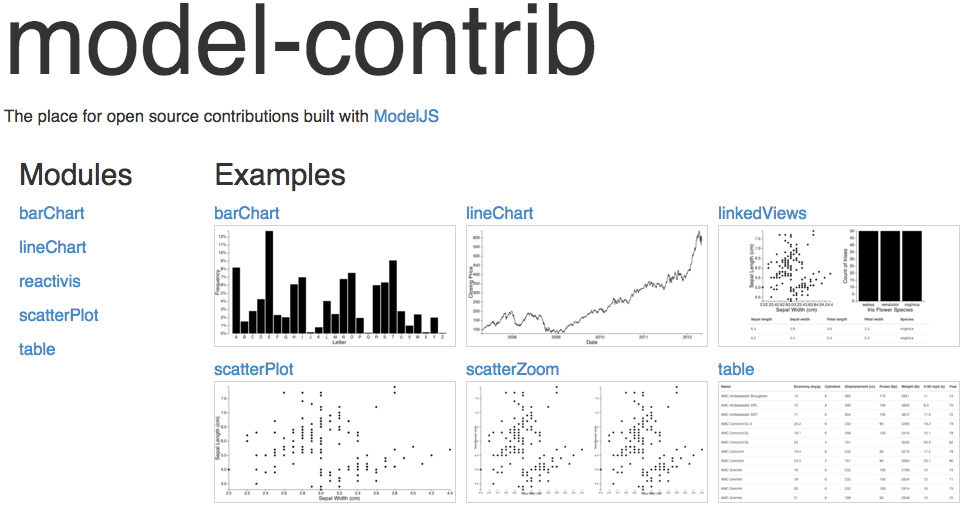
\includegraphics[width=\figureWidth]{figs/model-contrib.png}
  \caption [Model-Contrib Home Page]{The model-contrib project home page, showing a listing of reusable modules on the left and a gallery of examples with screenshots for each on the right.}
  \label{fig:lds}
\end{figure}

The Model-Contrib project is a playground for creating visualizations and reusable components using ModelJS. ModelJS contains the essence of reactive models, and all other contributions related to ModelJS belong in Model-Contrib. This includes example visualizations, visualizations with linked views, reusable visualization components. Other components such as Crossfilter integration and arbitrary SQL transformations are in Model-Contrib.

Model-Contrib includes an example viewer framework. This framework is responsible for displaying example screenshot thumbnails on the main model-contrib page, found at \verb`http://curran.github.io/model-contrib/#/`, and also for rendering the example detail pages. The example detail pages run the example inside the page using an iFrame, render the README Markdown to HTML, and display the syntax-highlighted code for each source file using CodeMirror. AngularJS is used to implement the example viewer client. PhantomJS and GraphicsMagick are used for generating the thumbnail images.

\section{Reactivis}
\verb`https://github.com/curran/reactivis`

The Reactivis project contains reusable reactive graphs that can be composed together to create reusable visualization components. In this project, there is also an implementation of reactive data flow graph computation and visualization.

\section{Overseer}
\verb`https://github.com/curran/overseer`

The Overseer project implements the runtime engine for dynamic configuration of visualizations. This project contains an implementation of the algorithm that computes the difference between two consecutive configuration states.

\section{UDC}
\verb`https://github.com/curran/udc`

The UDC repository contains a JavaScript implementation of the Universal Data Cube API. This API is capable of loading, integrating and querying data sets represented in the UDC format. In the UDC format, each data sets consists of a data table (CSV file) and a metadata (JSON file).

\section{UDC-Data}
\verb`https://github.com/curran/udc-data`

This repository contains example data sets represented using the UDC format. These data sets include the United Nations population data set, and the World Bank GDP data set.

% % %% Beginning of back matter
\backmatter  %% <--- mandatory

%%
%% We don't support endnotes

%%
%% A bibliography is required.
\interlinepenalty=10000  % prevent split bibliography entries
\bibliographystyle{umthesis}
\bibliography{dissertation}
\end{document}

%%% Local Variables: 
%%% mode: latex
%%% TeX-master: t
%%% End: 
